%% \documentclass[handout,t]{beamer} % HANDOUT
%% \documentclass[handout,notes=show,t]{beamer} % NOTES
\documentclass[t]{beamer} % SLIDES

\usetheme{SIGIL}
\usepackage{beamer-tools-sigil}

\input{lib/math}  % basic mathematical notation
\input{lib/stat}  % notation for probability theory and statistics
\input{lib/vector}% convenience macros for vectors and matrices

%%%
%%% local configuration adjustments
%%%

%%% You can change pre-defined colours here, override built-in macros from the
%%% style definition and standard library, as well as define macros needed by
%%% all local documents.

%%% e.g. adjust counterpoint (dark green) for data projectors where greens are
%%% far too bright, as well as green component of light colour and pure green
%%% (of course, it's a better solution to adjust the gamma settings of your monitor)
%%
%% \definecolor{counterpoint}{rgb}{.1, .3, 0}
%% \definecolor{light}{rgb}{.45, .3, .55}
%% \definecolor{puregreen}{rgb}{0, .35, 0}

%% ----- extra packages we need to load

\usepackage{tikz}
\usepackage{alltt}              % code examples with nicely formatted comments
\usepackage{rotating}


%% ----- author and copyright messages (so updates are automatically inserted into all files)
\newcommand{\sigilauthors}{%
  \author[SIGIL]{Designed by Stefan Evert\inst{1} and Marco Baroni\inst{2}}
  \institute[Evert \& Baroni]{
    \inst{1}Computational Corpus Linguistics Group\\
    Friedrich-Alexander-Universit�t Erlangen-N�rnberg, Germany
    \and
    \inst{2}Center for Mind/Brain Sciences (CIMeC)\\
    University of Trento, Italy
  }
}
\newcommand{\sigilcopyright}{%
  \date[sigil.r-forge.r-project.org]{%
    \primary{\footnotesize\url{http://SIGIL.r-forge.r-project.org/}}\\
    \light{\tiny Copyright \textcopyright\ 2007--2018 Evert \& Baroni}}
}

%% ----- automatically show TOC reminder at beginning of each subsection
\AtBeginSubsection[]
{
  \begin{frame}
    \frametitle{Outline}
    \tableofcontents[current,currentsubsection]
  \end{frame}
}

%% ----- some useful macros for the SIGIL course

\newenvironment{Rcode}[1][]{%
  \setbeamercolor{block title}{fg=counterpoint,bg=counterpoint!15!white}%
  \setbeamercolor{block body}{bg=counterpoint!5!white}\small%
  \begin{block}{#1}\begin{alltt}\ungap[1]}{%
      \ungap[1]\end{alltt}\end{block}} % \end{alltt} ... to deconfuse emacs

%% use \sbox{\Rbox} ... \usebox{\Rbox} to insert arbitray latex into Rcode environment
\newsavebox{\Rbox}

%% > plot(x,y)      \REM{this produces a scatterplot}
\newcommand{\REM}[2][\small]{\textsf{#1\color{primary}\# #2}}

%% nice colour for R output: \begin{Rout} .. \end{Rout}
\newenvironment{Rout}[1][\footnotesize]{%
  \begin{footnotesize}#1\color{secondary}\bfseries}{%
    \color{black}\mdseries\end{footnotesize}}

%% rotated column labels for table (to fit long text into narrow columns
\newcommand{\rotLabel}[2][60]{\begin{rotate}{#1}#2\end{rotate}}
 % local adjustments to configuration and macros

%%%%%%%%%%%%%%%%%%%%%%%%%%%%%%%%%%%%%%%%%%%%%%%%%%%%%%%%%%%%%%%%%%%%%%
%% Titlepage

\title[3a.\ Continuous Data: Description]{Unit 3: Descriptive Statistics for Continuous Data}
\subtitle{Statistics for Linguists with R -- A SIGIL Course}
\sigilauthors
\sigilcopyright
% \date[sigil.r-forge.r-project.org]{%
%   \light{\tiny \sigilcopyright}}

\begin{document}

\frame{\titlepage}

%%%%%%%%%%%%%%%%%%%%%%%%%%%%%%%%%%%%%%%%%%%%%%%%%%%%%%%%%%%%%%%%%%%%%%

\section*{Outline}
\frame{ 
  \frametitle{Outline}
  \tableofcontents
}

%%%%%%%%%%%%%%%%%%%%%%%%%%%%%%%%%%%%%%%%%%%%%%%%%%%%%%%%%%%%%%%%%%%%%%
\section{Introduction}

%%%%%%%%%%%%%%%%%%%%%%%%%%%%%%%%%%%%%%%%%%
\subsection{Categorical vs.\ numerical variables}

\begin{frame}
  \frametitle{Reminder: the library metaphor}
  % \framesubtitle{}

  \begin{itemize}
  \item In the library metaphor, we took random samples from an infinite
    population of tokens (words, VPs, sentences, \ldots)
  \item Relevant property is a binary (or \h{categorical}) classification
    \begin{itemize}
    \item active \vs passive VP or sentence (binary)
    \item instance of lemma TIME \vs some other word (binary)
    \item subcategorisation frame of verb token (itr, tr, ditr, p-obj, \ldots)
    \item part-of-speech tag of word token (50+ categories)
    \item[]
    \end{itemize}
    \pause
  \item Characterisation of population distribution is straightforward
    \begin{itemize}
    \item \h{binomial}: true proportion $\pi = 10\%$ of passive VPs,\\
      or relative frequency of TIME, e.g.\ $\pi = 2000\text{ pmw}$
    \item alternatively: specify redundant proportions $(\pi, 1-\pi)$,\\
      e.g.\ passive/active VPs $(.1, .9)$ or TIME/other $(.002, .998)$
    \item \h{multinomial}: multiple proportions $\pi_1 + \pi_2 + \dots + \pi_K
      = 1$,\\
      e.g.\ $(\pi_{\text{noun}} = .28, \pi_{\text{verb}} = .17, \pi_{\text{adj}} = .08, \ldots)$
    \end{itemize}
  \end{itemize}
\end{frame}

\begin{frame}
  \frametitle{Numerical properties}
  % \framesubtitle{}

  In many other cases, the properties of interest are \h{numerical}:

  \ungap
  \begin{columns}[t]
    \begin{column}{5cm}
      \begin{center}
        \hh{Population census}
        
        \gap\small
        \begin{tabular}{cccc}
          \toprule
          height & weight & shoes & sex\\
          \midrule
          178.18 &  69.52 &  39.5 & f \\
          160.10 &  51.46 &  37.0 & f \\
          150.09 &  43.05 &  35.5 & f \\
          182.24 &  63.21 &  46.0 & m \\
          169.88 &  63.04 &  43.5 & m \\
          185.22 &  90.59 &  46.5 & m \\
          166.89 &  47.43 &  43.0 & m \\
          162.58 &  54.13 &  37.0 & f \\
          \bottomrule
        \end{tabular}
      \end{center}
    \end{column}
    \begin{column}{5cm}
      \pause
      \begin{center}
        \hh{Wikipedia articles}

        \gap\small
        \begin{tabular}{cccc}
          \toprule
          tokens & types & TTR & avg len.\\
          \midrule
          696 & 251 & 2.773 & 4.532 \\
          228 & 126 & 1.810 & 4.488 \\
          390 & 174 & 2.241 & 4.251 \\
          455 & 176 & 2.585 & 4.412 \\
          399 & 214 & 1.864 & 4.301 \\
          297 & 148 & 2.007 & 4.399 \\
          755 & 275 & 2.745 & 3.861 \\
          299 & 171 & 1.749 & 4.524 \\
          \bottomrule
        \end{tabular}
      \end{center}
    \end{column}
  \end{columns}
  \addnote{Traditional example: populace of country, i.e.\ population of all
    inhabitants.  Properties of interest are physical measurements such as
    height, weight and shoe size; also age, income, IQ, size of household,
    \ldots}%
  \addnote{A more linguistic example: population of all English Wikipedia
    articles, with frequency statistics such as token count, type count,
    proportion of passives, token-type-ratio (TTR), avg.\ word length (wrt.\
    tokens or types), avg.\ frequency/familiarity class, \ldots}%
  \addnote{NB: both populations are finite, but very large (``practically
    infinite'').}%
  \addnote{Often there are also categorical properties, e.g.\ sex, level of
    education, Wikipedia category, has page won an award?, \ldots}%
\end{frame}

\begin{frame}
  \frametitle{Descriptive vs.\ inferential statistics}
  % \framesubtitle{}
  
  Two main tasks of ``classical'' statistical methods (numerical data):
  
  \gap\pause
  \begin{enumerate}
  \item \h{Descriptive statistics}
    \begin{itemize}
    \item compact description of the distribution of a (numerical) property in
      a very large or infinite population
    \item often by characteristic \hh{parameters} such as mean, variance,
      \ldots
    \item this was the original purpose of statistics in the 19th century
    \item[]
    \end{itemize}
    \pause
  \item \h{Inferential statistics}
    \begin{itemize}
    \item infer (aspects of) population distribution from a comparatively small
      random sample
    \item accurate estimates for level of uncertainty involved
    \item often by testing (and rejecting) some \hh{null hypothesis} $H_0$
    \end{itemize}
  \end{enumerate}
\end{frame}

%%%%%%%%%%%%%%%%%%%%%%%%%%%%%%%%%%%%%%%%%%
\subsection{Scales of measurement}

\begin{frame}
  \frametitle{Statisticians distinguish 4 scales of measurement}
  % \framesubtitle{}

  \textbf{Categorical data}
  \begin{enumerate}
  \item<2->[1.] \h{Nominal scale}: purely qualitative classification
    \begin{itemize}
    \item male \vs female, passive \vs active, POS tags, subcat frames
    \end{itemize}
  \item<3->[2.] \h{Ordinal scale}: ordered categories
    \begin{itemize}
    \item school grades A--E, social class, low/medium/high rating
    \end{itemize}
  \end{enumerate}

  \gap[.5]
  \textbf{Numerical data}
  \begin{enumerate}
  \item<4->[3.] \h{Interval scale}: meaningful comparison of differences
    \begin{itemize}
    \item temperature (\textdegree C), plausibility \& grammaticality ratings
    \end{itemize}
  \item<5->[4.] \h{Ratio scale}: comparison of magnitudes, absolute zero
    \begin{itemize}
    \item time, length/width/height, weight, frequency counts
    \end{itemize}
  \end{enumerate}

  \gap[.5]
  \onslide<6->
  Additional dimension: \h{discrete} \vs\ \h{continuous} numerical data
  \begin{itemize}
  \item[]
    \begin{itemize}
    \item discrete: frequency counts, rating $(1, \ldots, 7)$, shoe size, \ldots
    \item continuous: length, time, weight, temperature, \ldots
    \end{itemize}
  \end{itemize}
\end{frame}

\begin{frame}
  \frametitle{Quiz}
  %% \framesubtitle{}

  \onslide<+->
  \textbf{Which scale of measurement / data type is it?}
  
  \begin{itemize}
  \item<+-> subcategorisation frame
  \item<+-> reaction time (in psycholinguistic experiment)
  \item<+-> familiarity rating on scale $1, \ldots, 7$
  \item<+-> room number
  \item<+-> grammaticality rating: ``*'', ``??'', ``?'' or ``ok''
  \item<+-> magnitude estimation of plausibility (graphical scale)
  \item<+-> frequency of passive VPs in text 
  \item<+-> relative frequency of passive VPs
  \item<+-> token-type-ratio (TTR) and average word length (Wikipedia)
  \end{itemize}

  \onslide<+->\gap
  \hand\ in this unit: continuous numerical variables on ratio scale
\end{frame}

%%%%%%%%%%%%%%%%%%%%%%%%%%%%%%%%%%%%%%%%%%%%%%%%%%%%%%%%%%%%%%%%%%%%%%
\section{Descriptive statistics}

%%%%%%%%%%%%%%%%%%%%%%%%%%%%%%%%%%%%%%%%%%
\subsection{Characteristic measures}

\begin{frame}[fragile]
  \frametitle{The task}
  % \framesubtitle{}

  \begin{itemize}
  \item Census data from small country of \emph{Ingary} with $m =$~502,202
    inhabitants.  The following properties were recorded:
    \begin{itemize}
    \item body height in cm
    \item weight in kg
    \item shoe size in Paris points (Continental European system)
    \item sex (\emph{male}, \emph{female})
    \end{itemize}
  \item Frequency statistics for $m =$~1,429,649 Wikipedia articles:
    \begin{itemize}
    \item token count
    \item type count
    \item token-type ratio (TTR)
    \item average word length (across tokens)
    \end{itemize}
  \item[\hand] Describe / summarise these data sets (continuous variables)
  \end{itemize}

  \pause
  \begin{alltt}\small
    > library(SIGIL)
    > FakeCensus <- simulated.census()
    > WackypediaStats <- simulated.wikipedia()
  \end{alltt}
\end{frame}

\begin{frame}[fragile]
  \frametitle{Characteristic measures: central tendency}
  % \framesubtitle{}

  \begin{itemize}
  \item How would you describe body heights with a single number?%
    \pause
    \[
    \text{\h{mean}} \quad \mu = \frac{ x_1 + \dots + x_m }{ m }
    = \frac{1}{m} \sum_{i=1}^m x_i
    \]
  \item Is this intuitively sensible? Or are we just used to it?
  \end{itemize}

  \gap\pause
  \begin{alltt}
    > mean(FakeCensus$height)\begin{Rout}
    [1] 170.9781  \end{Rout}
    > mean(FakeCensus$weight)\begin{Rout}
    [1] 65.28917  \end{Rout}
    > mean(FakeCensus$shoe.size)\begin{Rout}
    [1] 41.49712  \end{Rout}
  \end{alltt} % $

  \addnote{We will see a (partial) mathematical justification later today.}%
\end{frame}

\begin{frame}
  \frametitle{Characteristic measures: variability (spread)}
  % \framesubtitle{}

  \begin{itemize}
  \item Average weight of 65.3 kg not very useful if we have to design an
    elevator for 10 persons or a chair that doesn't collapse:\\
    We need to know if everyone weighs close to 65~kg, or whether the typical
    range is 40--100~kg, or whether it is even larger.
  \item Measure of spread: \hh{minimum} and \hh{maximum}, here 30--196~kg
  \item We're more interested in the ``typical'' range of values without the
    most extreme cases
  \item Average variability based on \h{error} $x_i - \mu$ for each individual
    shows how well the mean $\mu$ describes the entire population
  \end{itemize}

  \only<beamer:2| handout:0>{
    \[
    \frac{1}{m} \sum_{i=1}^m (x_i - \mu) = 0
    \]
  }
  \only<beamer:3| handout:0>{
    \[
    \frac{1}{m} \sum_{i=1}^m \abs{x_i - \mu}
    \quad\text{is mathematically inconvenient}
    \]
  }
  \only<beamer:4| handout:1>{
    \[
    \text{\h{variance}}\quad
    \sigma^2 = \frac{1}{m} \sum_{i=1}^m (x_i - \mu)^2
    \]
  }
\end{frame}

\begin{frame}
  \frametitle{Characteristic measures: variability (spread)}
  % \framesubtitle{}

  \[
  \text{\h{variance}}\quad
  \sigma^2 = \frac{1}{m} \sum_{i=1}^m (x_i - \mu)^2
  \]
  \begin{itemize}
  \item[\hand] Do you remember how to calculate this in R?
    \begin{itemize}
    \item<2-> height: \secondary{$\mu = 171.00$}, $\sigma^2 = 199.50$%
      \only<3->{, \secondary{$\sigma = 14.12$}}
    \item<2-> weight: \secondary{$\mu = 65.29$}, $\sigma^2 = 306.72$%
      \only<3->{, \secondary{$\sigma = 17.51$}}
    \item<2-> shoe size: \secondary{$\mu = 41.50$}, $\sigma^2 = 21.70$%
      \only<3->{, \secondary{$\sigma = 4.66$}}
    \item[]
    \end{itemize}
  \item<3-> Mean and variance are not on a comparable scale\\
    \so \h{standard deviation} (\h{s.d.}) $\sigma = \sqrt{\sigma^2}$
    \begin{itemize}
    \item[]
    \end{itemize}
  \item<3-> NB: still gives more weight to larger errors!
  \end{itemize}
\end{frame}

\begin{frame}
  \frametitle{Characteristic measures: higher moments}
  % \framesubtitle{}

  \begin{itemize}
  \item Mean based on $(x_i)^1$ is also known as a ``first moment'',\\
    variance based on $(x_i)^2$ as a ``second moment''
  \item The third moment is called \h{skewness}
    \[
    \gamma_1 = \frac{1}{m} \sum_{i=1}^m \left( 
      \frac{x_i - \mu}{\sigma}
    \right)^3
    \]
    and measures the asymmetry of a distribution
  \item The fourth moment (\h{kurtosis}) measures ``bulginess''
    \begin{itemize}
    \item[]\pause
    \end{itemize}
  \item How useful are these characteristic measures?
    \begin{itemize}
    \item Given the mean, s.d., skewness, \ldots, can you tell how many people
      are taller than 190~cm, or how many weigh $\approx 100$~kg?
    \item Such measures mainly used for computational efficiency, and even
      this required an elaborate procedure in the 19th century
    \end{itemize}
  \end{itemize}
\end{frame}

%%%%%%%%%%%%%%%%%%%%%%%%%%%%%%%%%%%%%%%%%%
\subsection{Histogram \& density}

\begin{frame}
  \frametitle{The shape of a distribution: discrete data}
  \framesubtitle{Discrete numerical data can be tabulated and plotted}

  \ungap
  \begin{center}
    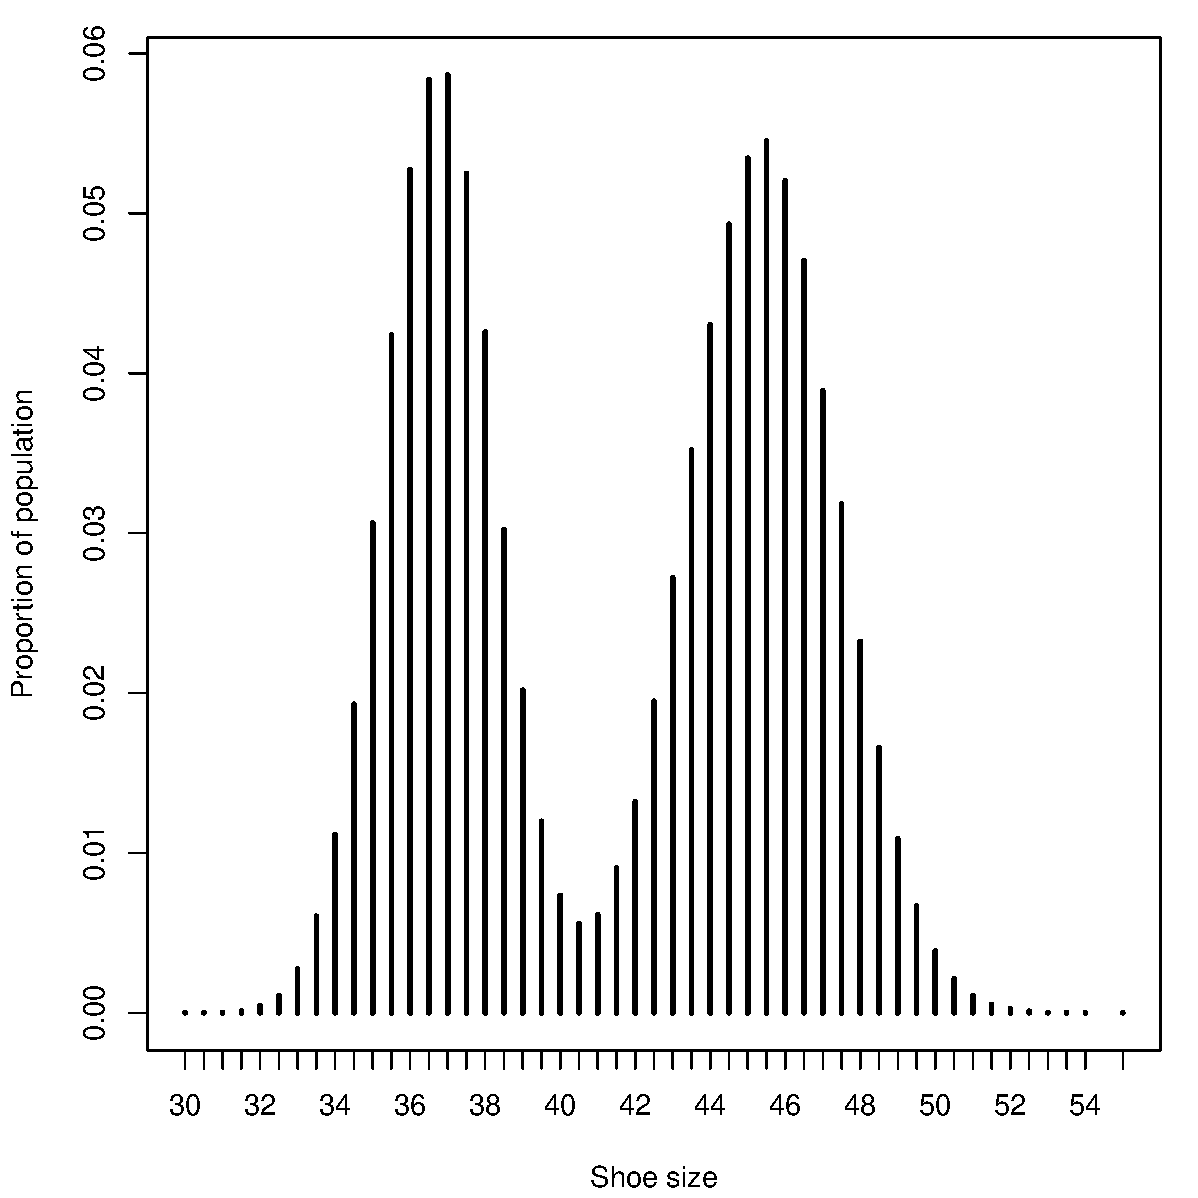
\includegraphics[width=7cm]{img/ingary_shoesize_table}
  \end{center}
\end{frame}

\begin{frame}
  \frametitle{The shape of a distribution: histogram for continuous data}
  \framesubtitle{Continuous data must be collected into bins \so histogram}

  \ungap[2.5]
  \begin{center}
    \begin{tabular}{cc}
      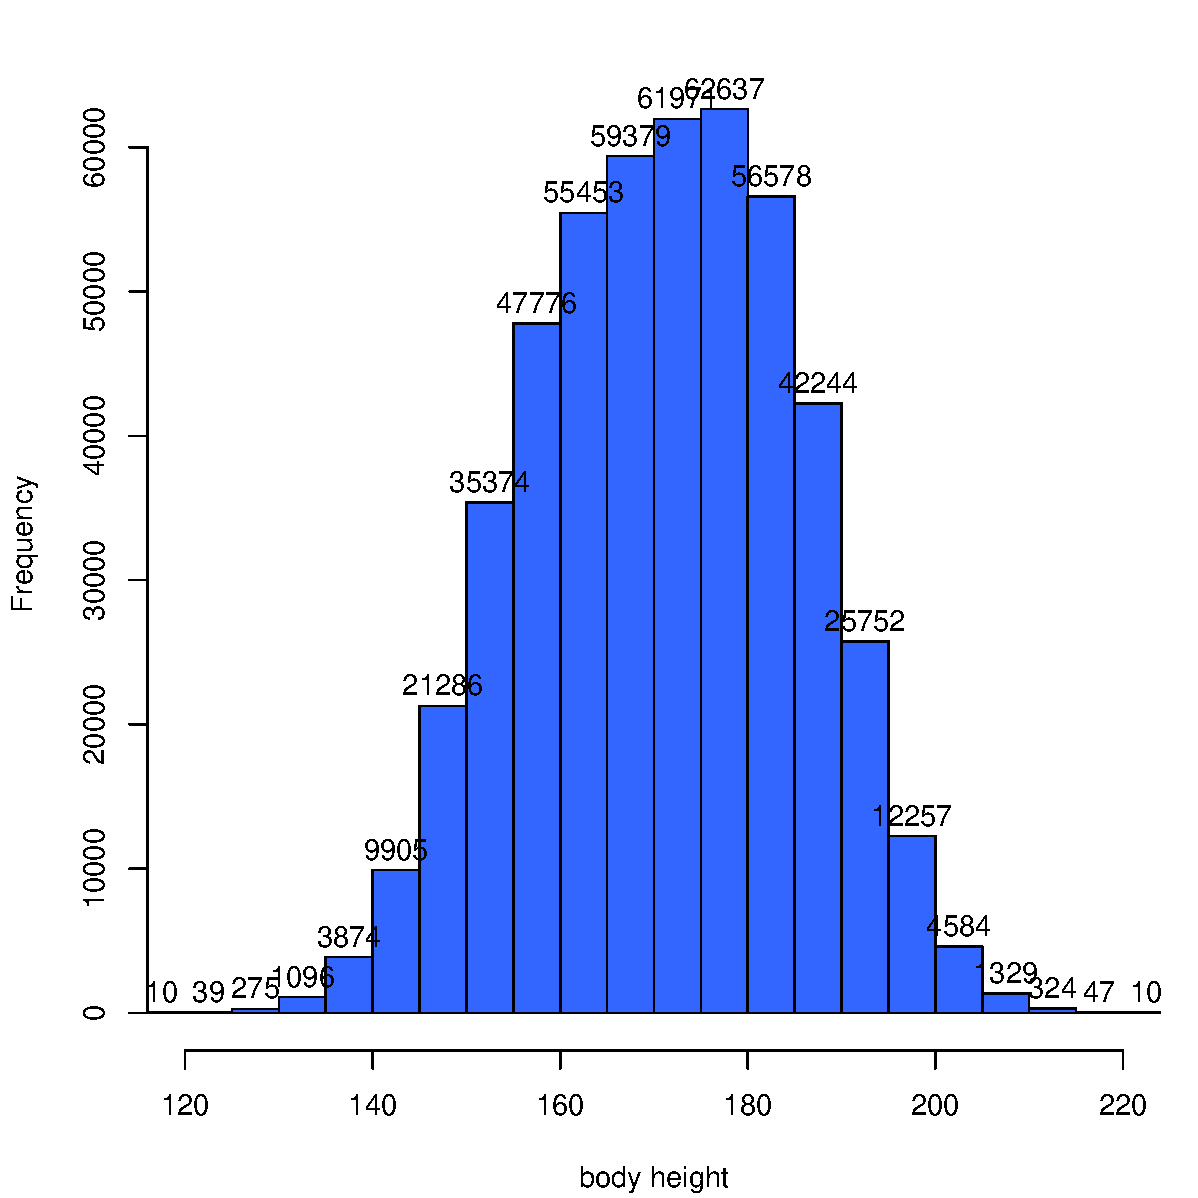
\includegraphics[width=55mm]{img/ingary_hist_freq_1} &
      \visible<2->{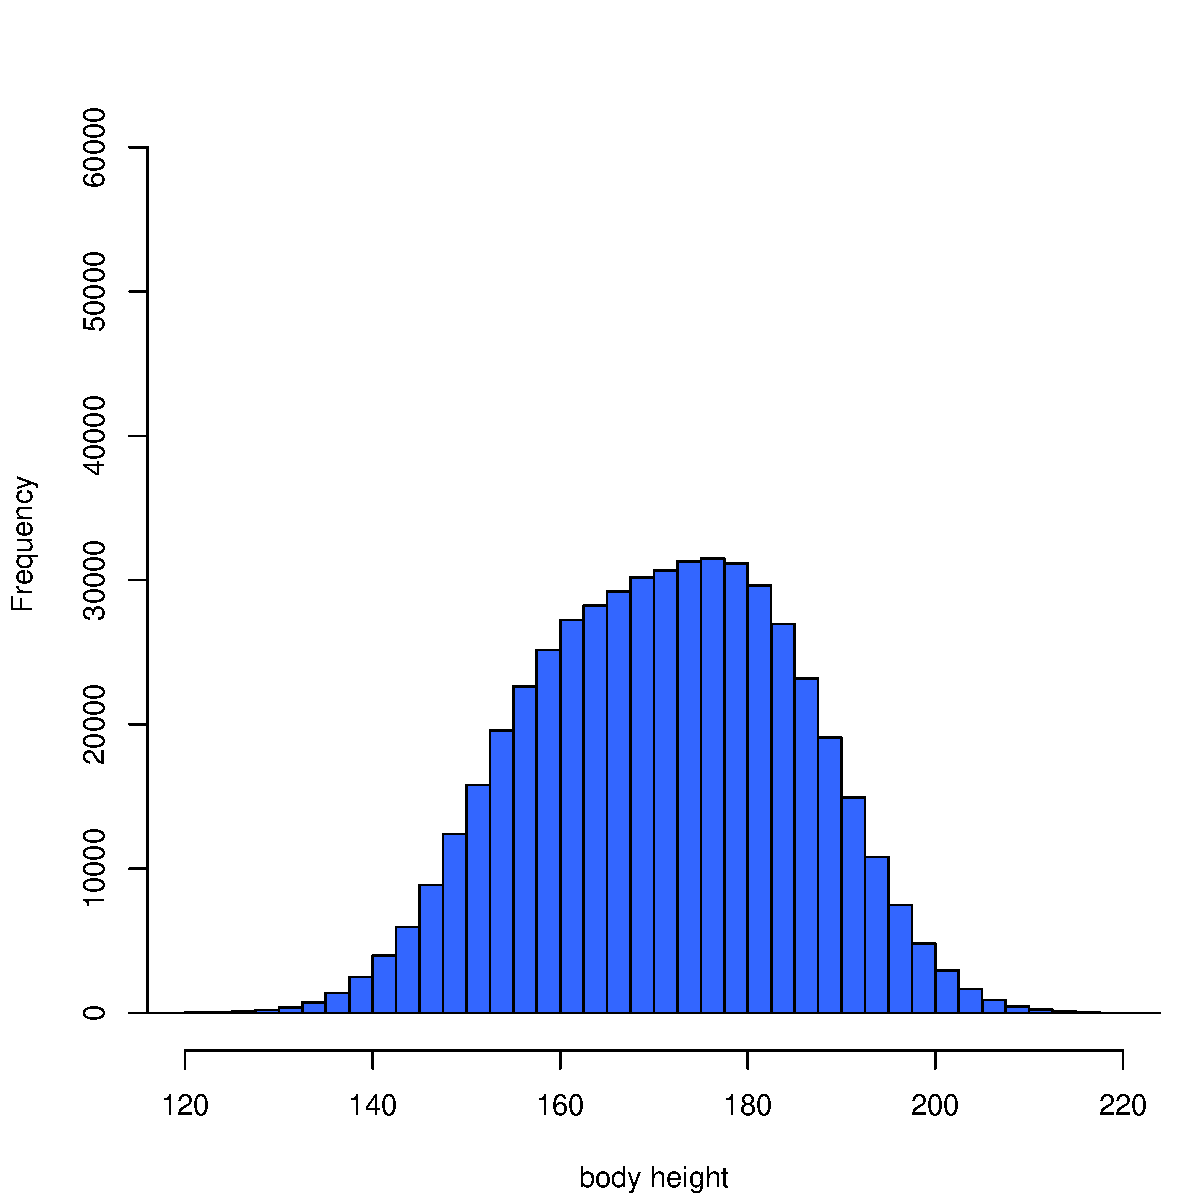
\includegraphics[width=55mm]{img/ingary_hist_freq_2}}
    \end{tabular}
  \end{center}

  \ungap[1]
  \begin{itemize}
  \item No two people have \emph{exactly} the same body height, weight, \ldots
  \item<2-> Frequency counts (= y-axis scale) depend on number of bins
  \end{itemize}
\end{frame}

\begin{frame}
  \frametitle{The shape of a distribution: histogram for continuous data}
  \framesubtitle{Continuous data must be collected into bins \so histogram}

  \ungap[2.5]
  \begin{center}
    \begin{tabular}{cc}
      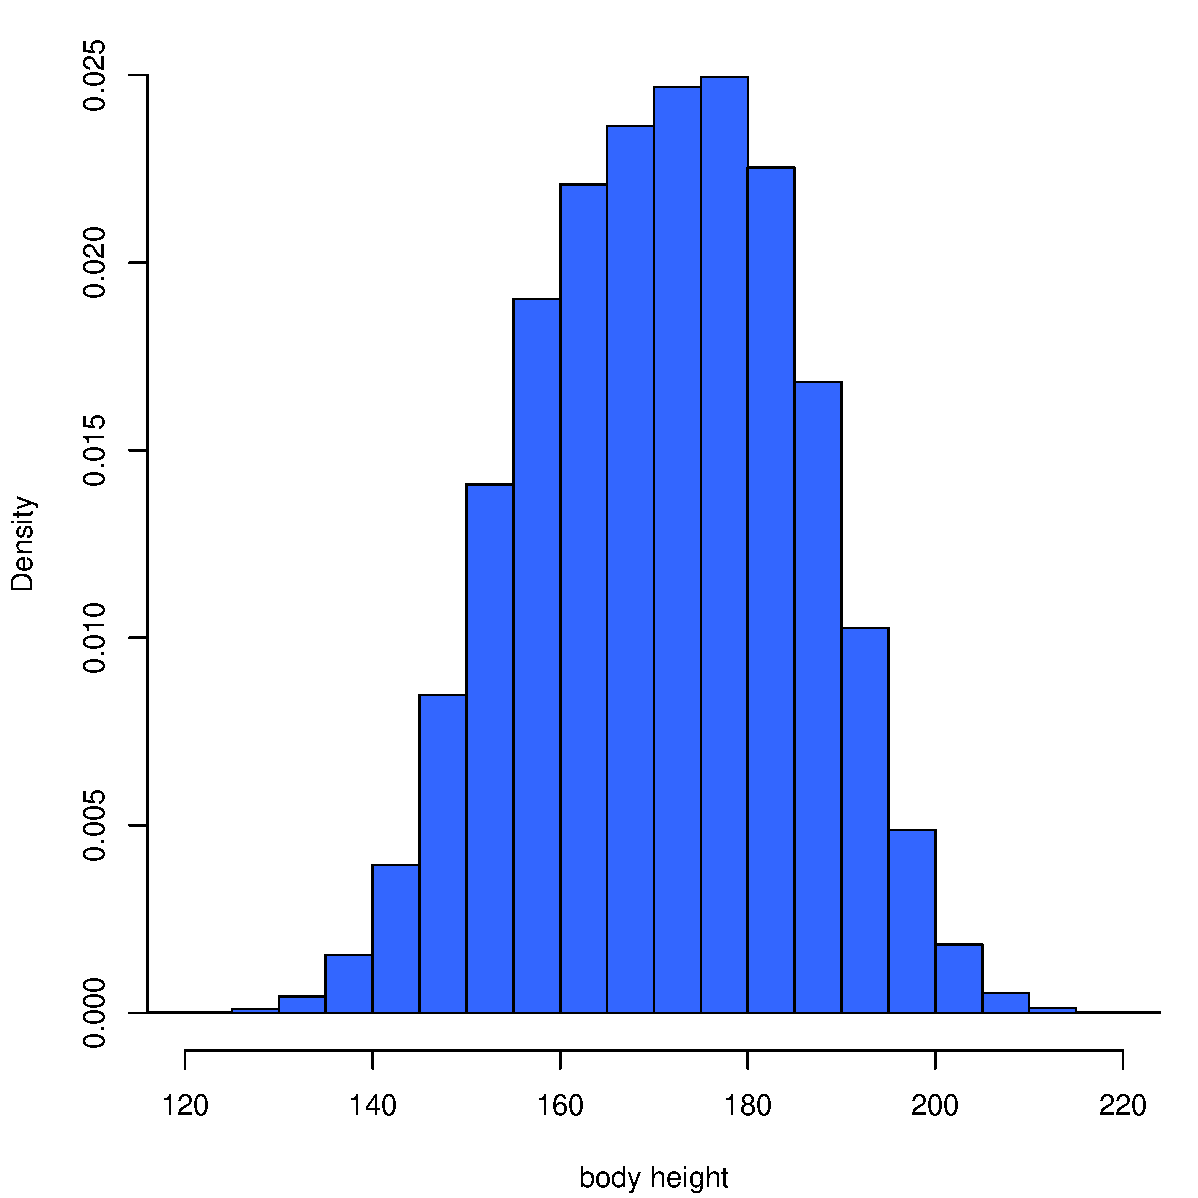
\includegraphics[width=55mm]{img/ingary_hist_1} &
      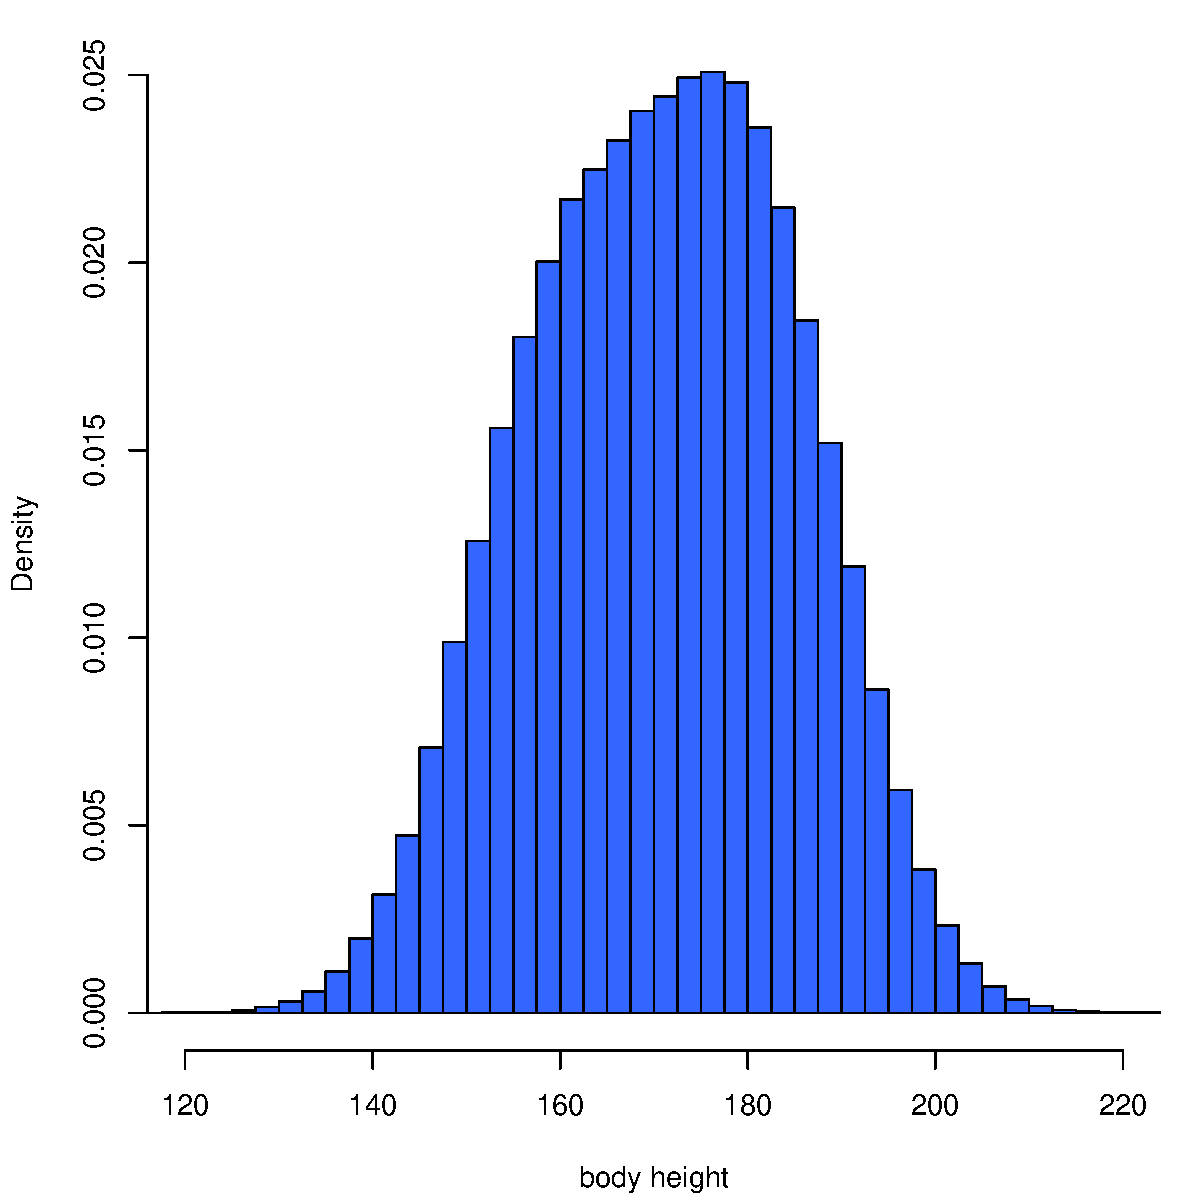
\includegraphics[width=55mm]{img/ingary_hist_2}
    \end{tabular}
  \end{center}

  \ungap[1]
  \begin{itemize}
  \item \h{Density} scale is comparable for different numbers of bins
  \item Area of histogram bar $\equiv$ relative frequency in population
  \end{itemize}
\end{frame}

\begin{frame}
  \frametitle{Refining histograms: the density function}

  \ungap[1]
  \begin{center}
    \only<beamer:1| handout:0>{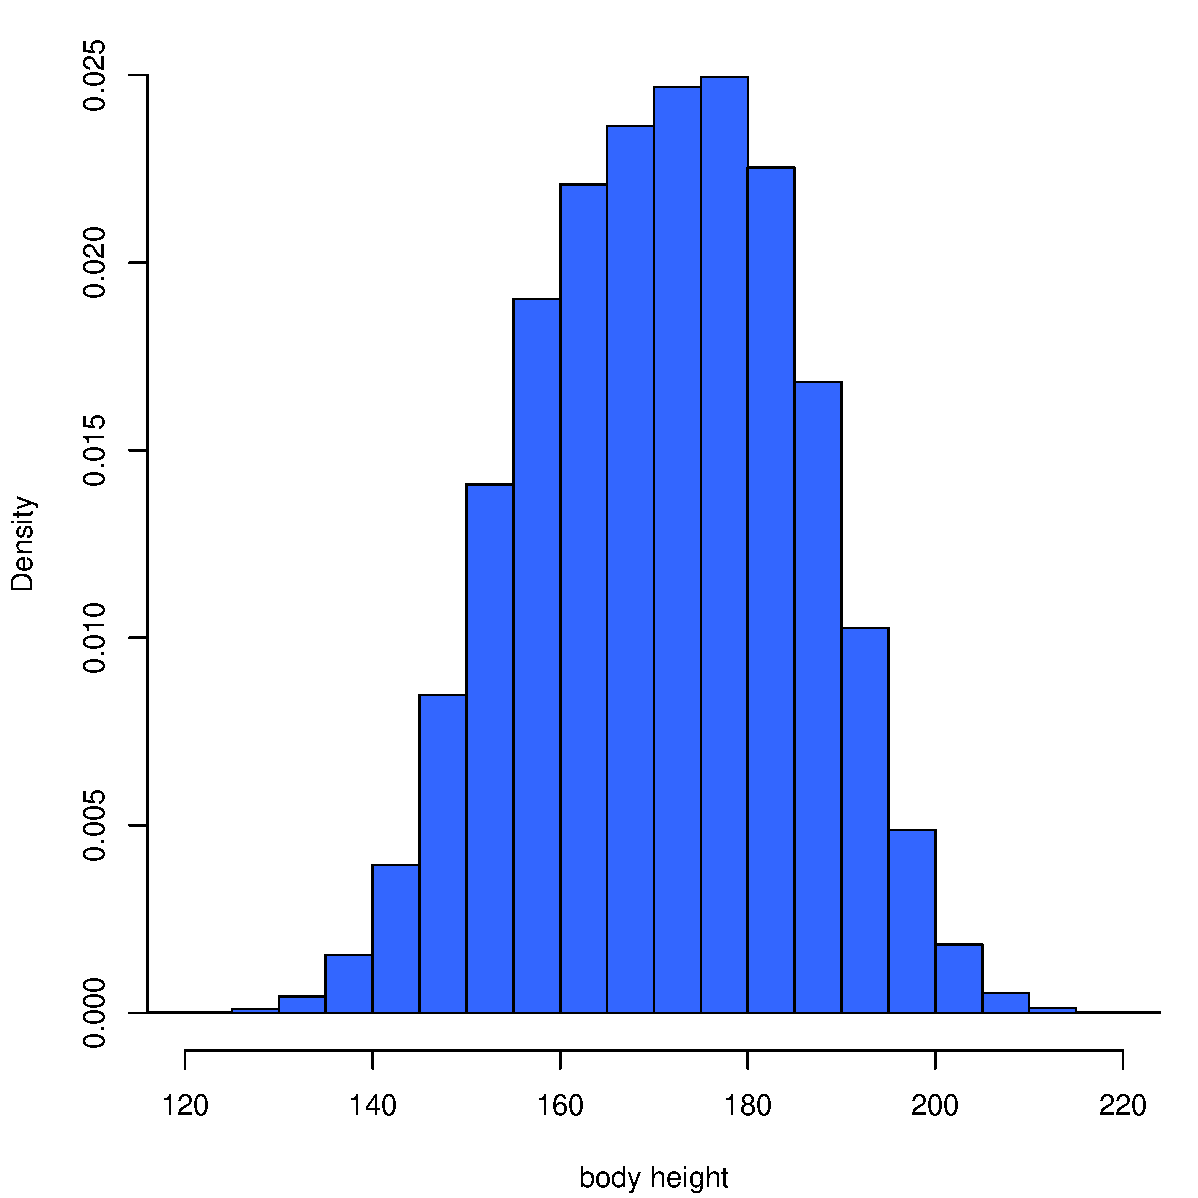
\includegraphics[width=65mm]{img/ingary_hist_1}}%
    \only<beamer:2| handout:0>{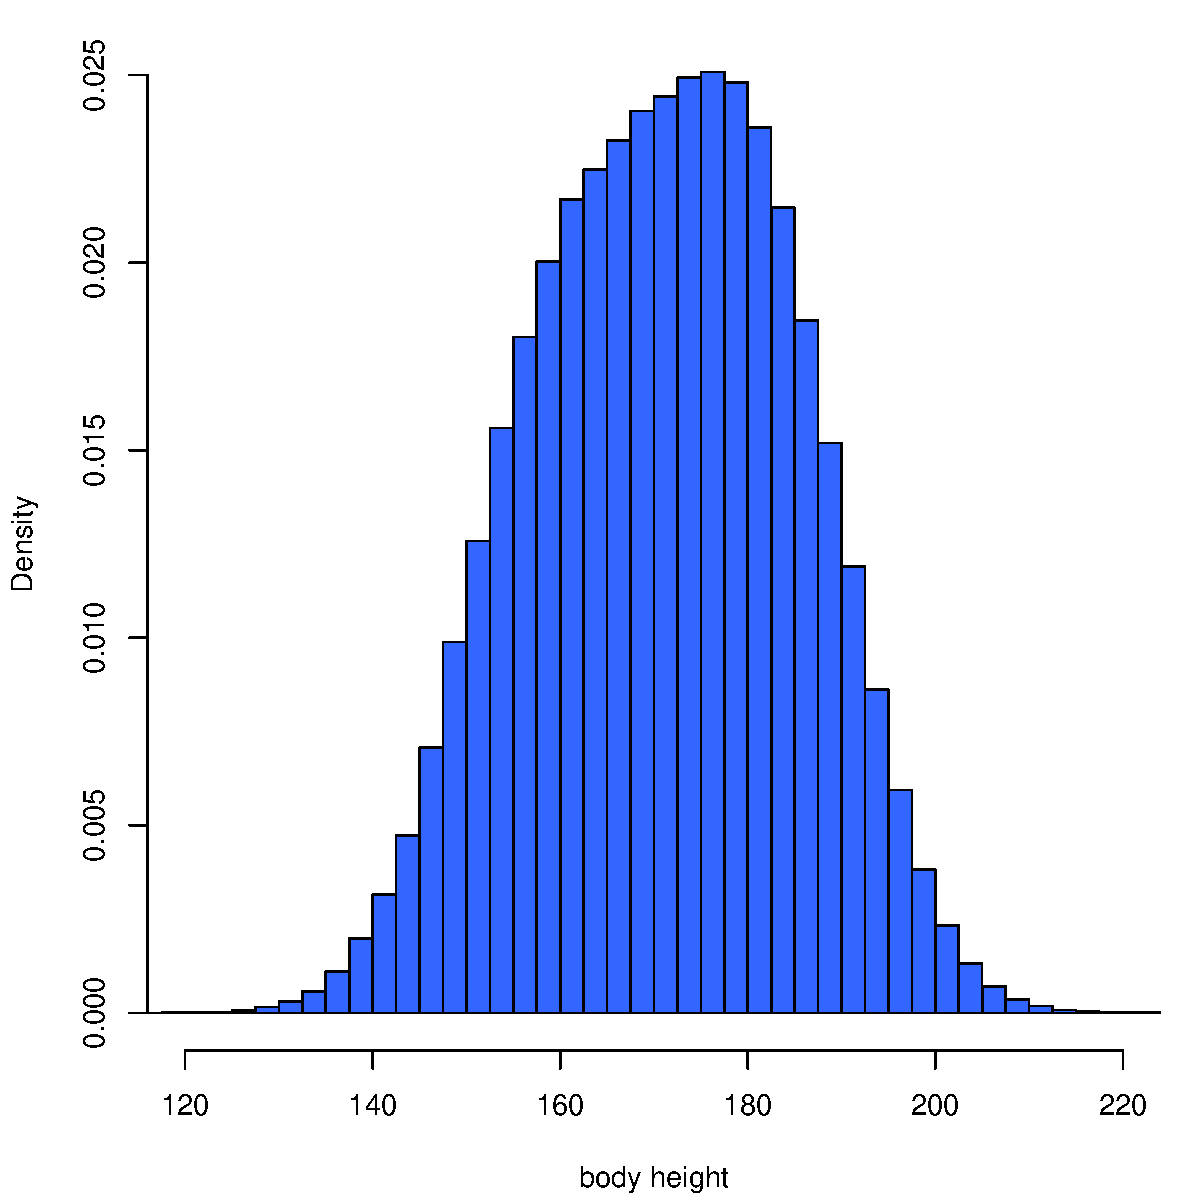
\includegraphics[width=65mm]{img/ingary_hist_2}}%
    \only<beamer:3| handout:0>{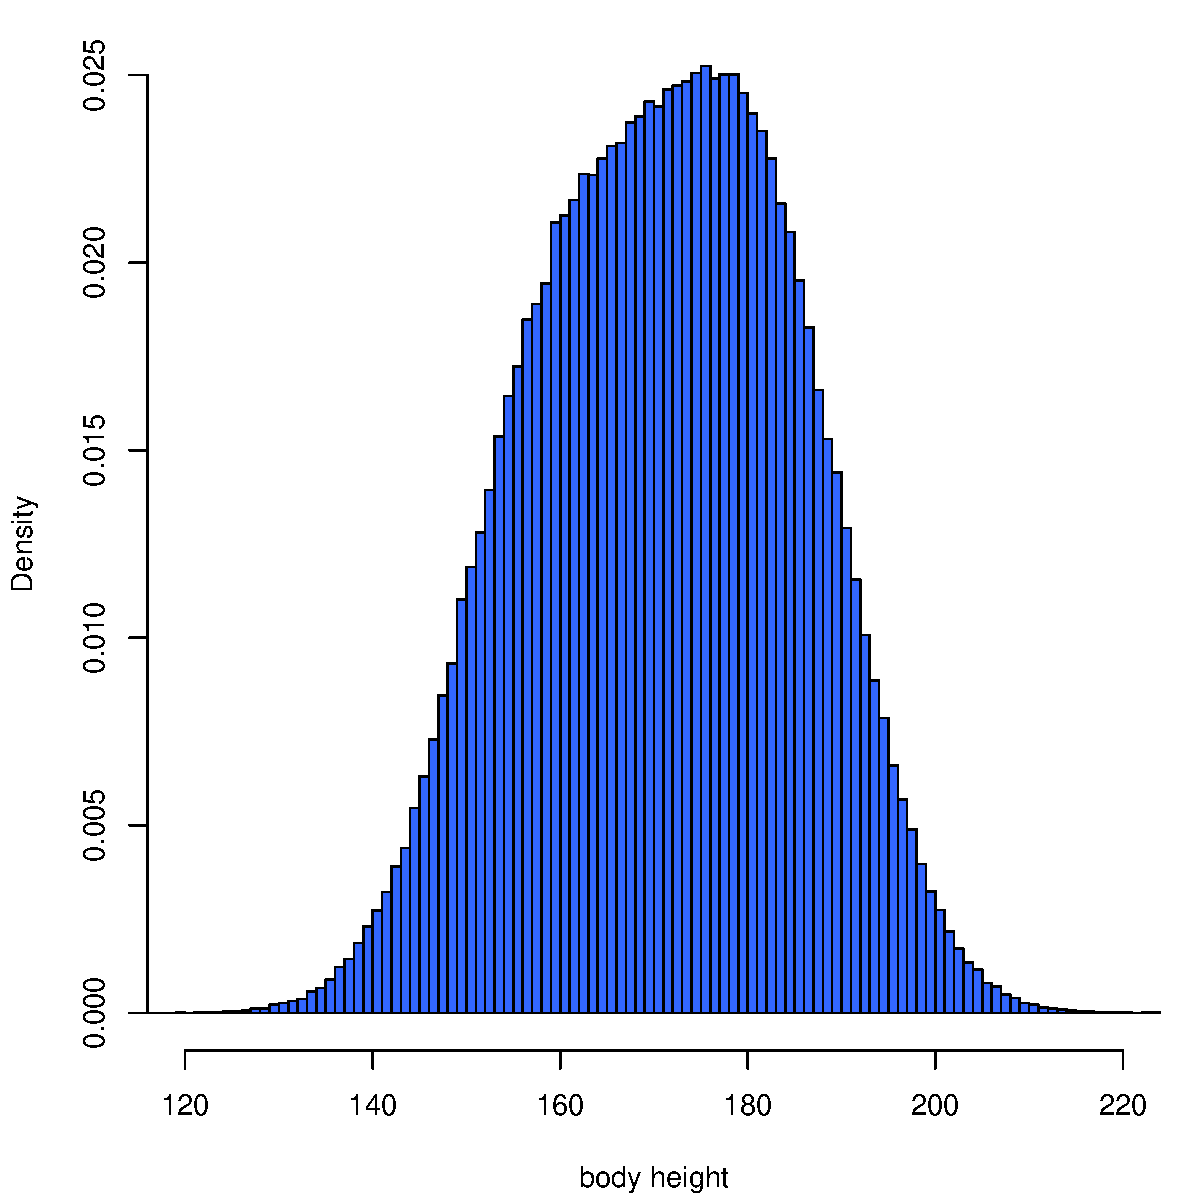
\includegraphics[width=65mm]{img/ingary_hist_3}}%
    \only<beamer:4| handout:0>{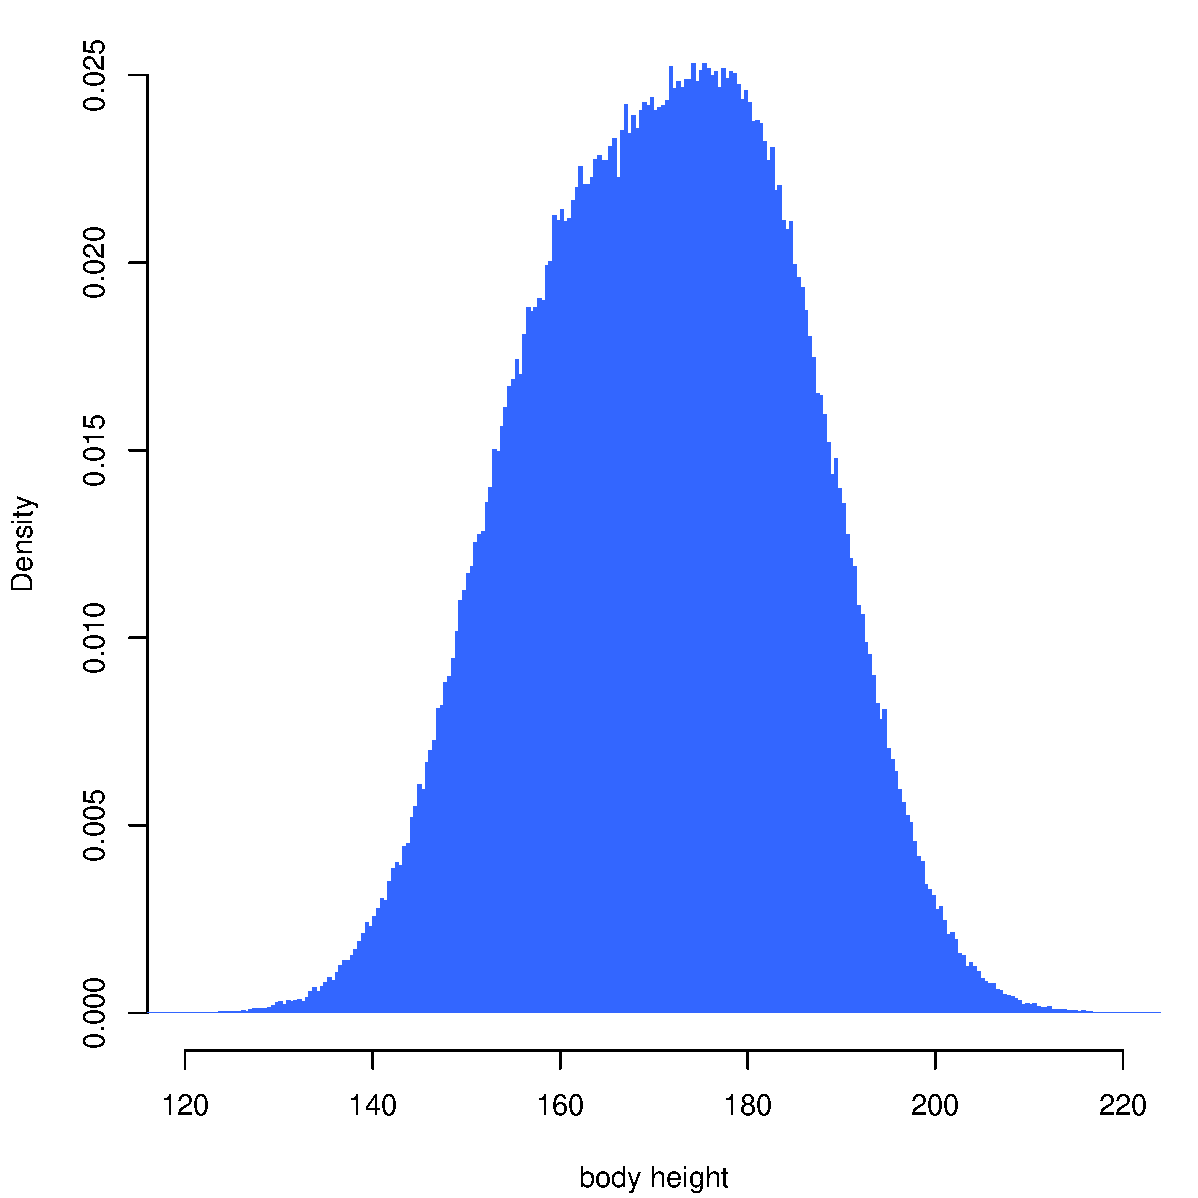
\includegraphics[width=65mm]{img/ingary_hist_4}}%
    \only<beamer:5| handout:1>{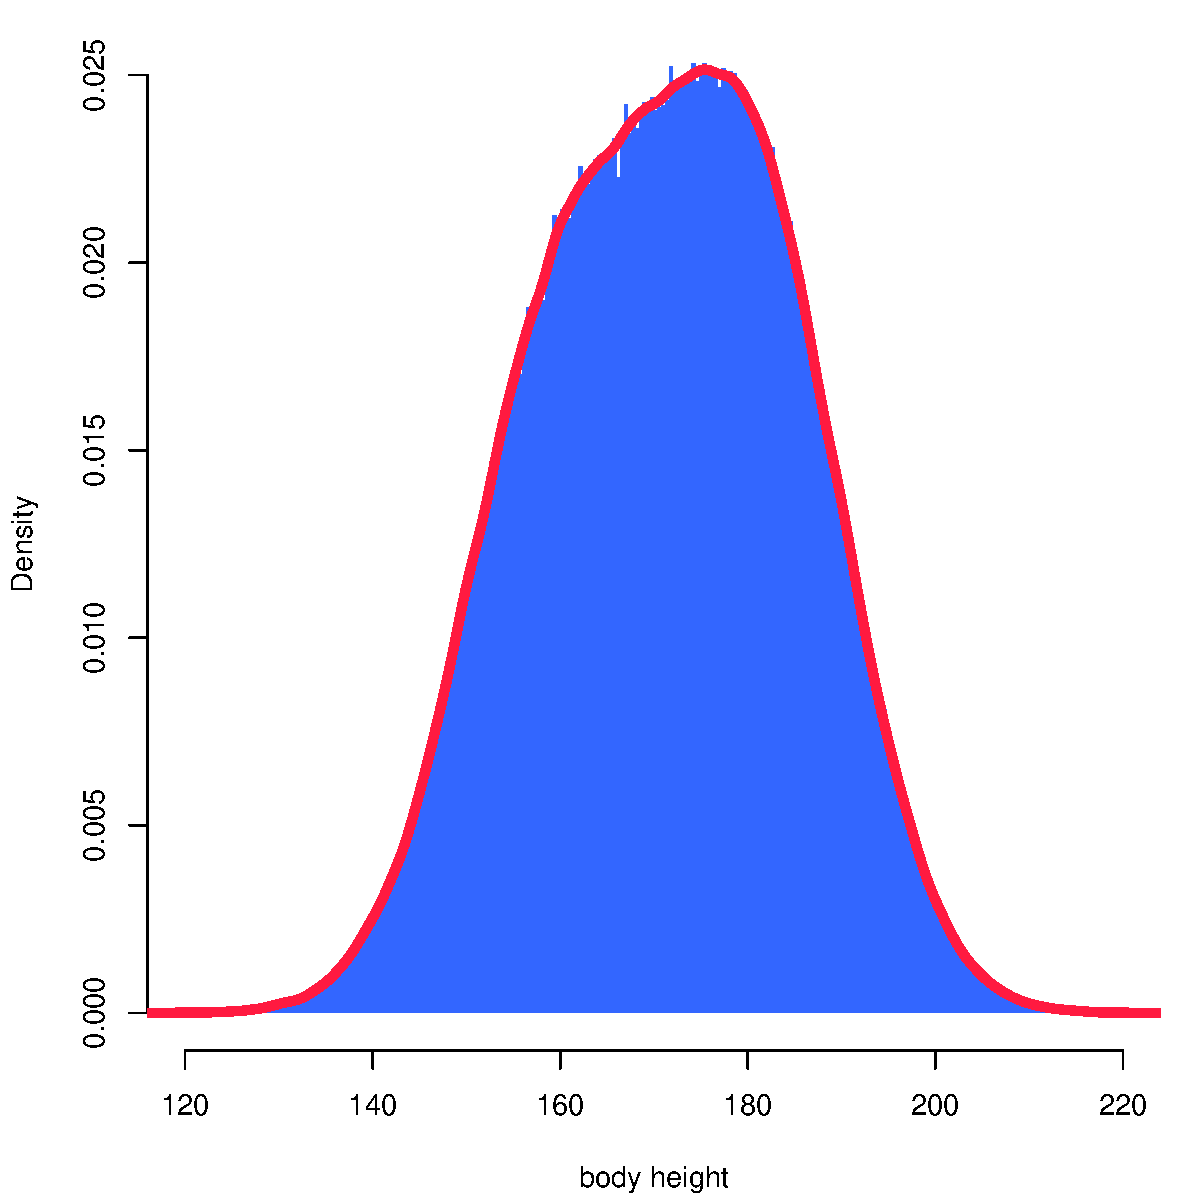
\includegraphics[width=65mm]{img/ingary_hist_4_curve}}
  \end{center}

  \ungap[1]
  \begin{itemize}
  \item<5-> Contour of histogram = \h{density function}
  \end{itemize}
\end{frame}

%%%%%%%%%%%%%%%%%%%%%%%%%%%%%%%%%%%%%%%%%%
\subsection{Random variables \& expectations}

\begin{frame}
  \frametitle{Formal mathematical notation}
  % \framesubtitle{}

  \begin{itemize}
  \item \h{Population} $\Omega = \set{\omega_1, \omega_2, \ldots, \omega_m}$
    with $m\approx \infty$
    \begin{itemize}
    \item item $\omega_k$ = person, Wikipedia article, word (lexical
      RT), \ldots
    \end{itemize}
  \item<2-> For each item, we are interested in several properties (e.g.\ height,
    weight, shoe size, sex) called \h{random variables} (\h{r.v.})
    \begin{itemize}
    \item height $X: \Omega\to \setR^+$ with $X(\omega_k) =$ height of person $\omega_k$
    \item weight $Y: \Omega\to \setR^+$ with $Y(\omega_k) =$ weight of person $\omega_k$
    \item sex $G: \Omega\to \set{0,1}$ with $G(\omega_k) = 1$ iff
      $\omega_k$ is a woman
    \item[\hand] formally, a r.v.\ is a (usually real-valued) function over
      $\Omega$
    \end{itemize}
  \item<3-> \h{Mean}, \h{variance}, etc.\ computed for each random variable:
    \begin{small}
    \begin{align*}
      \mu_X &= \frac{1}{m} \sum_{\omega\in \Omega} X(\omega) \eqcolon \Exp{X}
      && \text{\h{expectation}} \\
      \sigma^2_X &= \frac{1}{m} \sum_{\omega\in \Omega} \bigl( X(\omega) - \mu \bigr)^2 
      \eqcolon \Var{X}  && \text{\h{variance}} \\
      &= \Expscale{(X - \mu)^2}
    \end{align*}
    \end{small}
  \end{itemize}
  \ungap[1.5]
  \addnote{Term \emph{random variable} makes sense if you think of e.g.\ $X$
    as the height of a randomly selected person; it yields a different value
    each time you pick a new person.}%
  \addnote{Point out the numerical $\set{0,1}$ coding of a binary categorical
    variable.  If numerical coding is used for multinomial variables, each
    category hast to be coded by a separate indicator variable; otherwise,
    spurious relations between the categories would be implied.}%
  \addnote{Keep in mind that $\mu\in \setR$ is a fixed real number, so the
    variance sum can be calculated as an expectation over (a function of) $X$.}%
\end{frame}

\begin{frame}
  \frametitle{Working with random variables}
  % \framesubtitle{}

  \begin{itemize}
  \item<1-> $X'(\omega) \coloneq \bigl(X(\omega) - \mu\bigr)^2$ defines new r.v.\
    $X': \Omega\to \setR$
    \begin{itemize}
    \item[\hand] any function $f(X)$ of a r.v.\ is itself a random variable
    \end{itemize}
  \item<1-> The expectation is a \hh{linear functional} on r.v.:
    \begin{itemize}
    \item $\Exp{X + Y} = \Exp{X} + \Exp{Y}$ for $X, Y: \Omega\to \setR$
    \item $\Exp{r\cdot X} = r\cdot \Exp{X}$ for $r\in \setR$
    \item $\Exp{a} = a$ for constant r.v.\ $a\in \setR$ (additional property)
    \end{itemize}
  \item<2-> These rules enable us to simplify the computation of $\sigma^2_X$:
    \begin{small}
    \begin{align*}
      \sigma^2_X &= \Var{X} = \Expscale{(X - \mu_X)^2}
      = \Expscale{X^2 - 2\mu_X X + \mu^2_X}\\
      &= \Exp{X^2} - 2\mu_X \underbrace{\Exp{X}}_{= \mu_X} + \mu^2_X
      = \Exp{X^2} - \mu^2_X
    \end{align*}
    \end{small}
  \item<3-> Random variables and probabilities: r.v.\ $X$ describes outcome of
    picking a random $\omega\in \Omega$ \so \hh{sampling distribution}
    \begin{small}
    \[
    \p{a\leq X\leq b} = \frac{1}{m} \bigabs{\setdef{\omega\in \Omega}{a \leq
        X(\omega) \leq b}}
    \]
    \end{small}
  \end{itemize}
\end{frame}

\begin{frame}
  \frametitle{A justification for the mean}
  % \framesubtitle{}
  
  \begin{itemize}
  \item<1-> $\sigma^2_X$ tells us how well the r.v.\ $X$ is characterised by $\mu_X$
  \item<1-> More generally, $\Expscale{(X-a)^2}$ tells us how well $X$ is
    characterised by some real number $a\in\setR$
  \item<2-> The best single value we can give for $X$ is the one that minimises
    the average squared error:
    \[
    \Expscale{(X-a)^2} = \Exp{X^2} - 2 a \underbrace{\Exp{X}}_{= \mu_X} + a^2
    \]
  \item<3-> It is easy to see that a minimum is achieved for $a = \mu_X$
    \begin{itemize}
    \item[\hand] The quadratic error term in our definition of $\sigma^2_X$
      guarantees that there is always a unique minimum.  This would not have
      been the case e.g.\ with $\abs{X - a}$ instead of $(X - a)^2$.
    \end{itemize}
  \end{itemize}
\end{frame}

\begin{frame}
  \frametitle{How to compute the expectation of a discrete variable}
  % \framesubtitle{}

  \begin{itemize}
  \item Population distribution of a \h{discrete} variable is fully described
    by giving the relative frequency of each possible value $t\in \setR$:
    \[
    \pi_t = \p{X = t}
    \]
    \ungap[2]\onslide<2->
    \begin{align*}
      \Exp{X} &= \sum_{\omega\in\Omega} \frac{X(\omega)}{m}
      = \underbrace{\sum_t \sum_{X(\omega)=t}}_{\text{group by value of $X$}}
      \!\!\!\!\! \frac{t}{m}
      = \sum_t t \sum_{X(\omega)=t} \frac{1}{m} \\
      &= \sum_t t\cdot \frac{\abs{X(\omega)=t}}{m} = \sum_t t\cdot \pi_t
      = \sum_t t\cdot \p{X=t}
    \end{align*}
  \item<3-> The second moment $\Exp{X^2}$ needed for $\Var{X}$ can also be
    obtained in this way from the population distribution:
    \[
    \Exp{X^2} = \sum_t t^2\cdot \p{X=t}
    \]
  \end{itemize}
\end{frame}

\begin{frame}
  \frametitle{How to compute the expectation of a continuous variable}
  % \framesubtitle{}

  \begin{itemize}
  \item Population distribution of \h{continuous} variable can be described by
    its \hh{density function} $g: \setR\to [0, \infty]$
    \begin{itemize}
    \item keep in mind that $\p{X=t} = 0$ for almost every value $t\in\setR$:
      nobody is \emph{exactly} 172.3456789 cm tall!
    \end{itemize}
  \end{itemize}
  
  \gap[.5]\pause
  \begin{columns}[c]
    \begin{column}{7.2cm}
      \begin{small}\raggedright
        Area under density curve between $a$ and $b$ = proportion of items
        $\omega\in\Omega$ with $a\leq X(\omega)\leq b$.
      \end{small}
      \[
      \p{a\leq X\leq b} = \int_a^b g(t) \dX{t} 
      \]
      \begin{small}\raggedright
        \visible<3->{Same reasoning as for discrete variable leads to:}
      \end{small}
    \end{column}
    \begin{column}{3cm}
      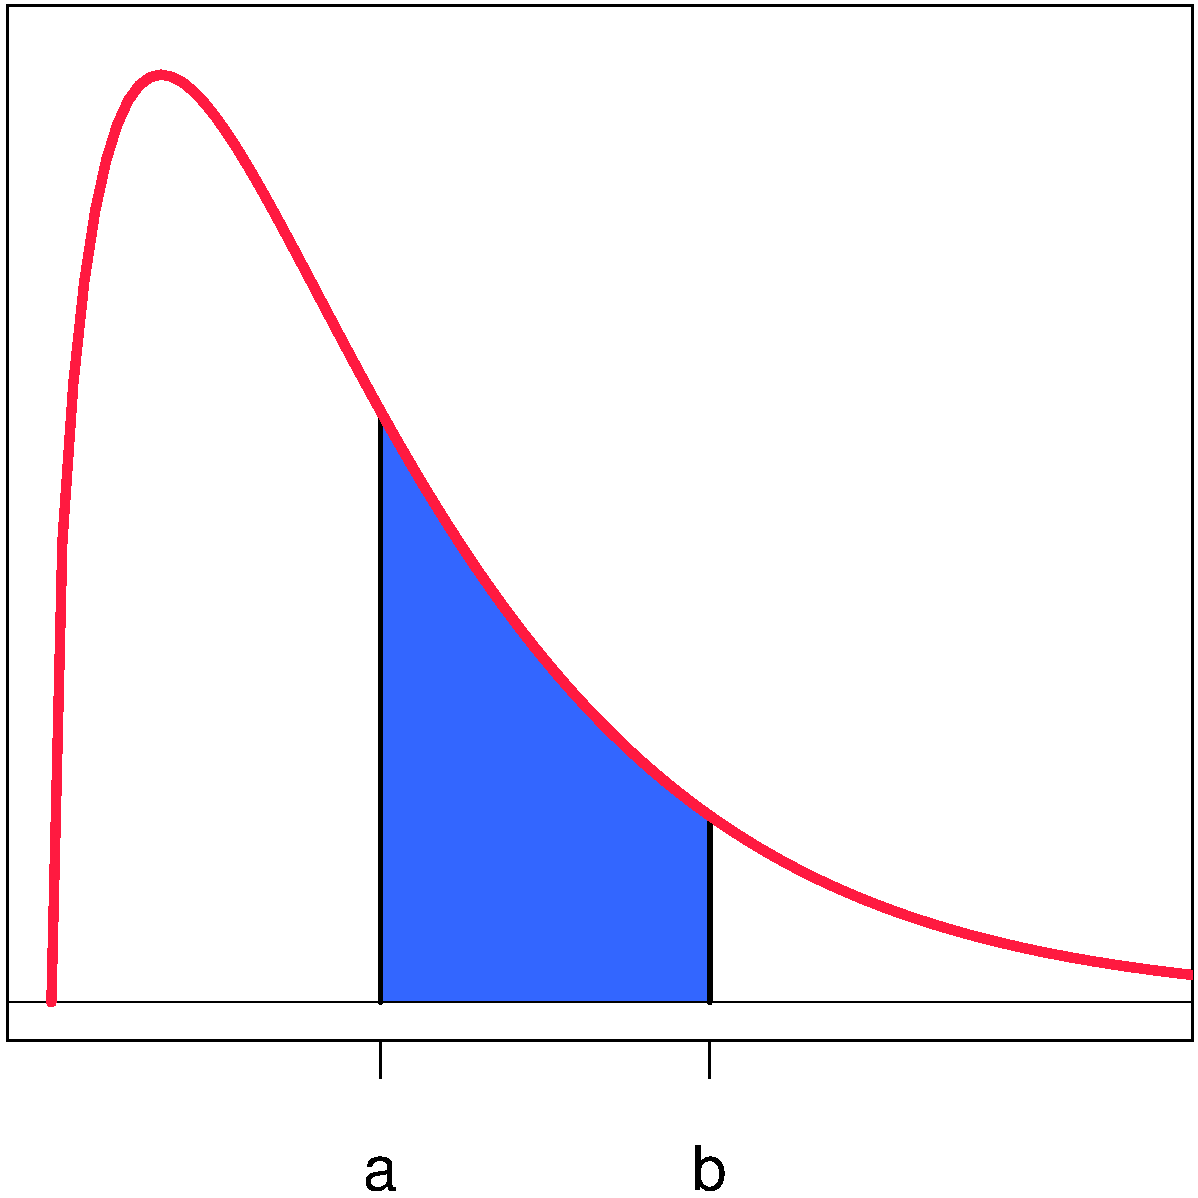
\includegraphics[width=3cm]{img/area_under_density}      
    \end{column}
  \end{columns}
  \pause
  \begin{align*}
    \Exp{X} &= \int_{-\infty}^{+\infty} t\cdot g(t) \dX{t} \qquad \text{and}\\
    \Exp{f(X)} &= \int_{-\infty}^{+\infty} f(t)\cdot g(t) \dX{t}
  \end{align*}

\end{frame}

%%%%%%%%%%%%%%%%%%%%%%%%%%%%%%%%%%%%%%%%%%%%%%%%%%%%%%%%%%%%%%%%%%%%%%
\section{Continuous distributions}

%%%%%%%%%%%%%%%%%%%%%%%%%%%%%%%%%%%%%%%%%%
\subsection{The shape of a distribution}

\begin{frame}
  \frametitle{Different types of continuous distributions}
  
  \ungap[1]
  \begin{center}
    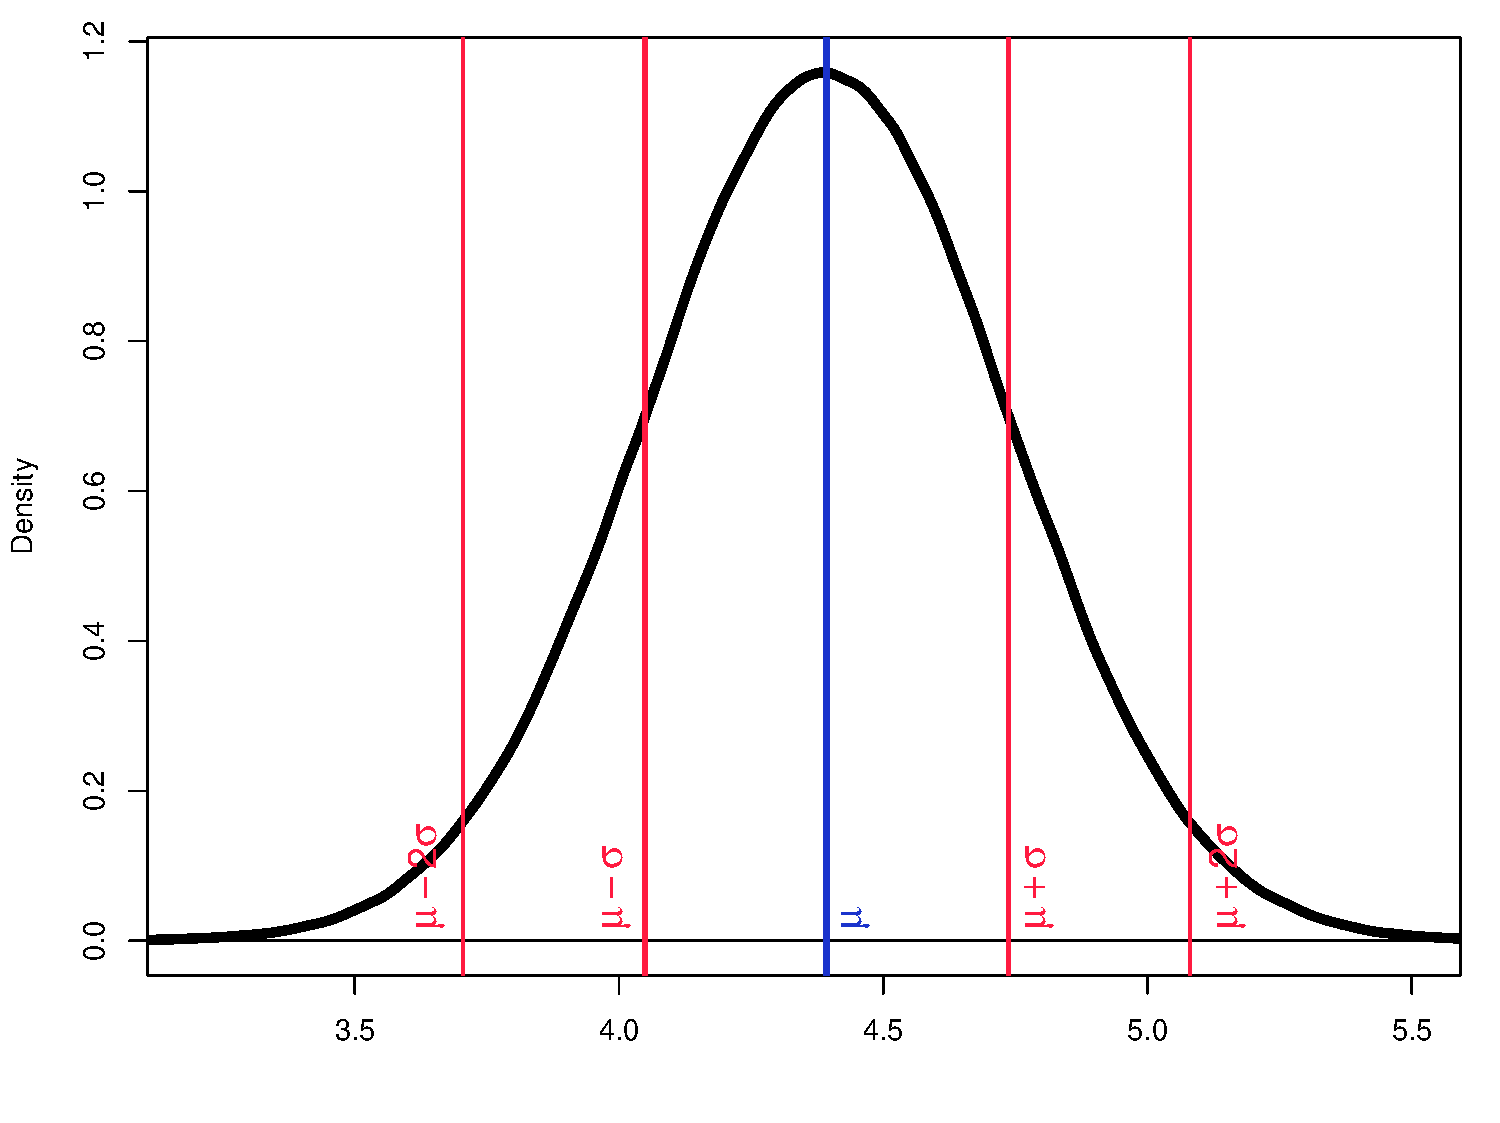
\includegraphics[width=9cm]{img/disttype_symmetric}

    \ungap[1]
    \h{symmetric, bell-shaped}
  \end{center}
\end{frame}

\begin{frame}
  \frametitle{Different types of continuous distributions}
  
  \ungap[1]
  \begin{center}
    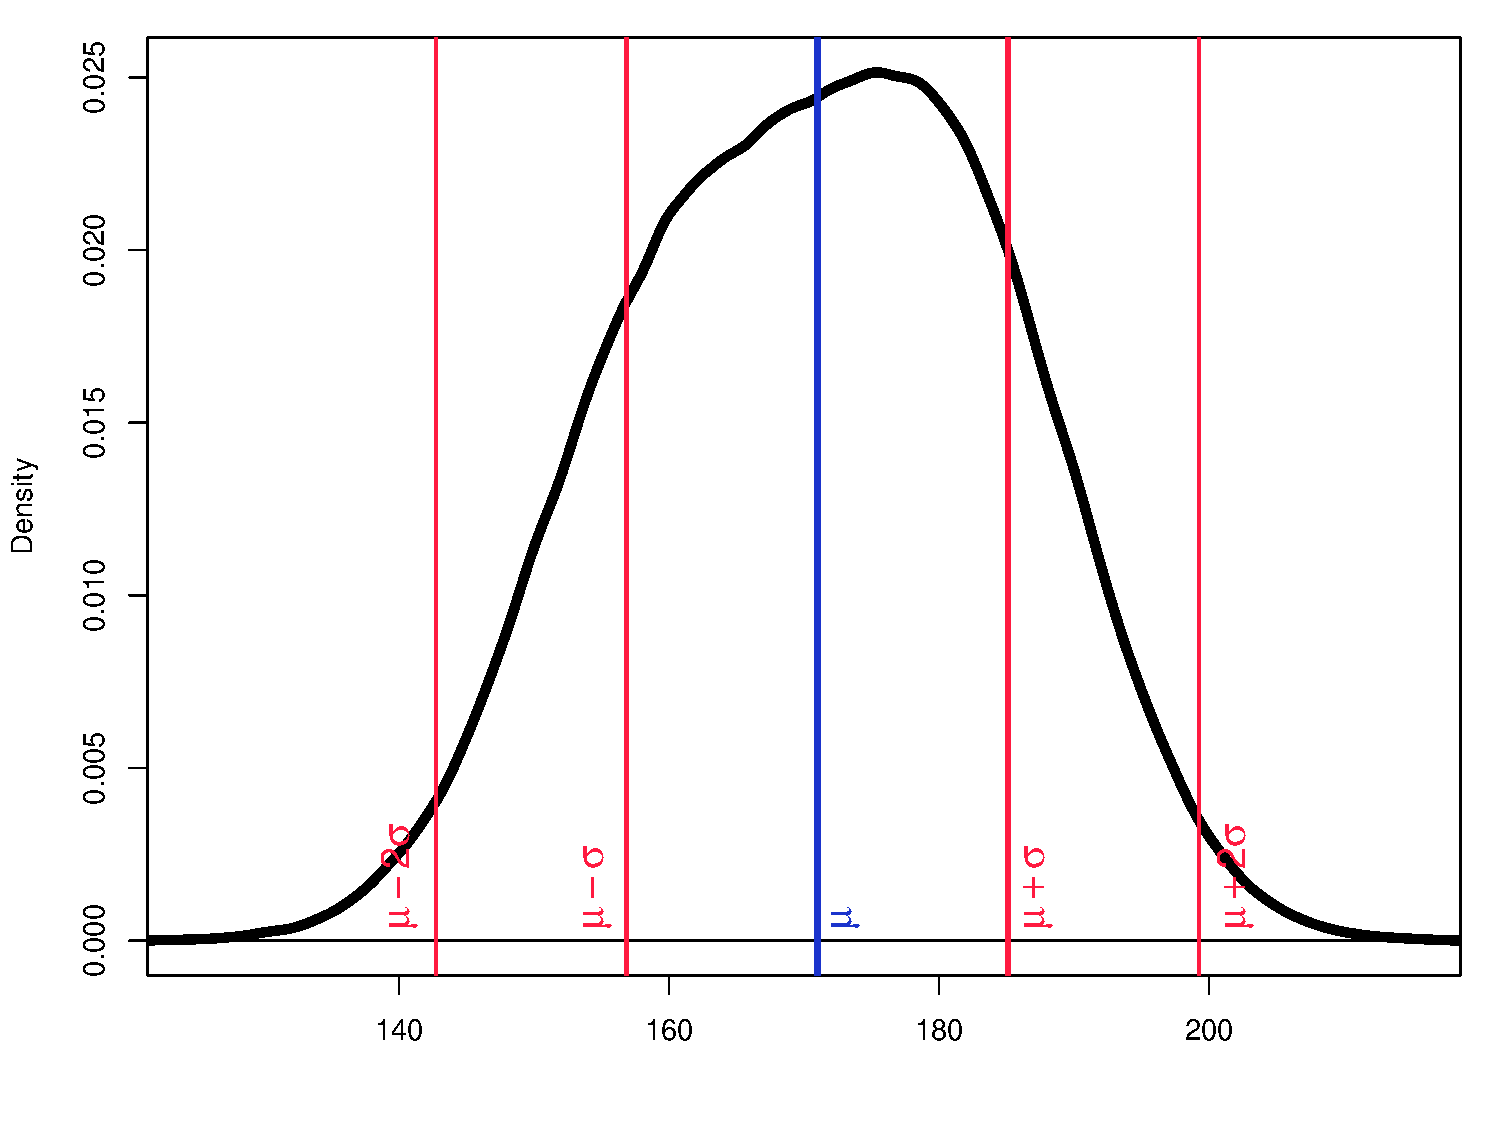
\includegraphics[width=9cm]{img/disttype_bulgy}

    \ungap[1]
    \h{symmetric, bulgy}
  \end{center}
\end{frame}

\begin{frame}
  \frametitle{Different types of continuous distributions}
  
  \ungap[1]
  \begin{center}
    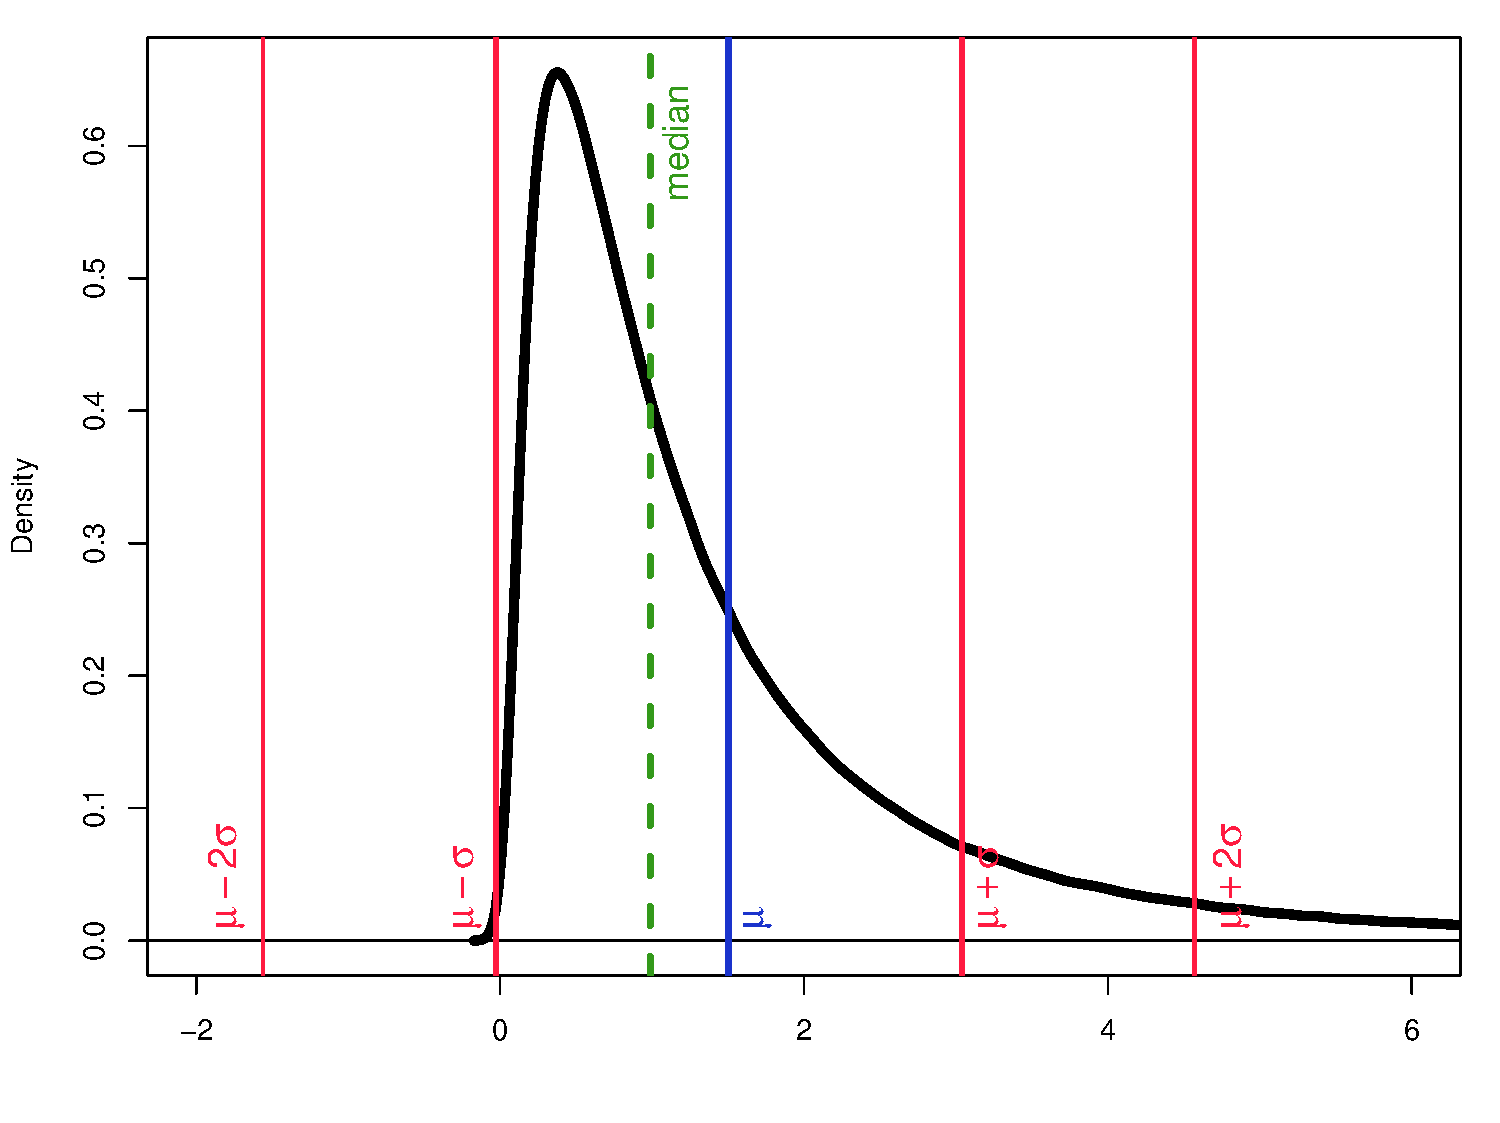
\includegraphics[width=9cm]{img/disttype_skewed}

    \ungap[1]
    \h{skewed} (median $\neq$ mean)
  \end{center}
\end{frame}

\begin{frame}
  \frametitle{Different types of continuous distributions}
  
  \ungap[1]
  \begin{center}
    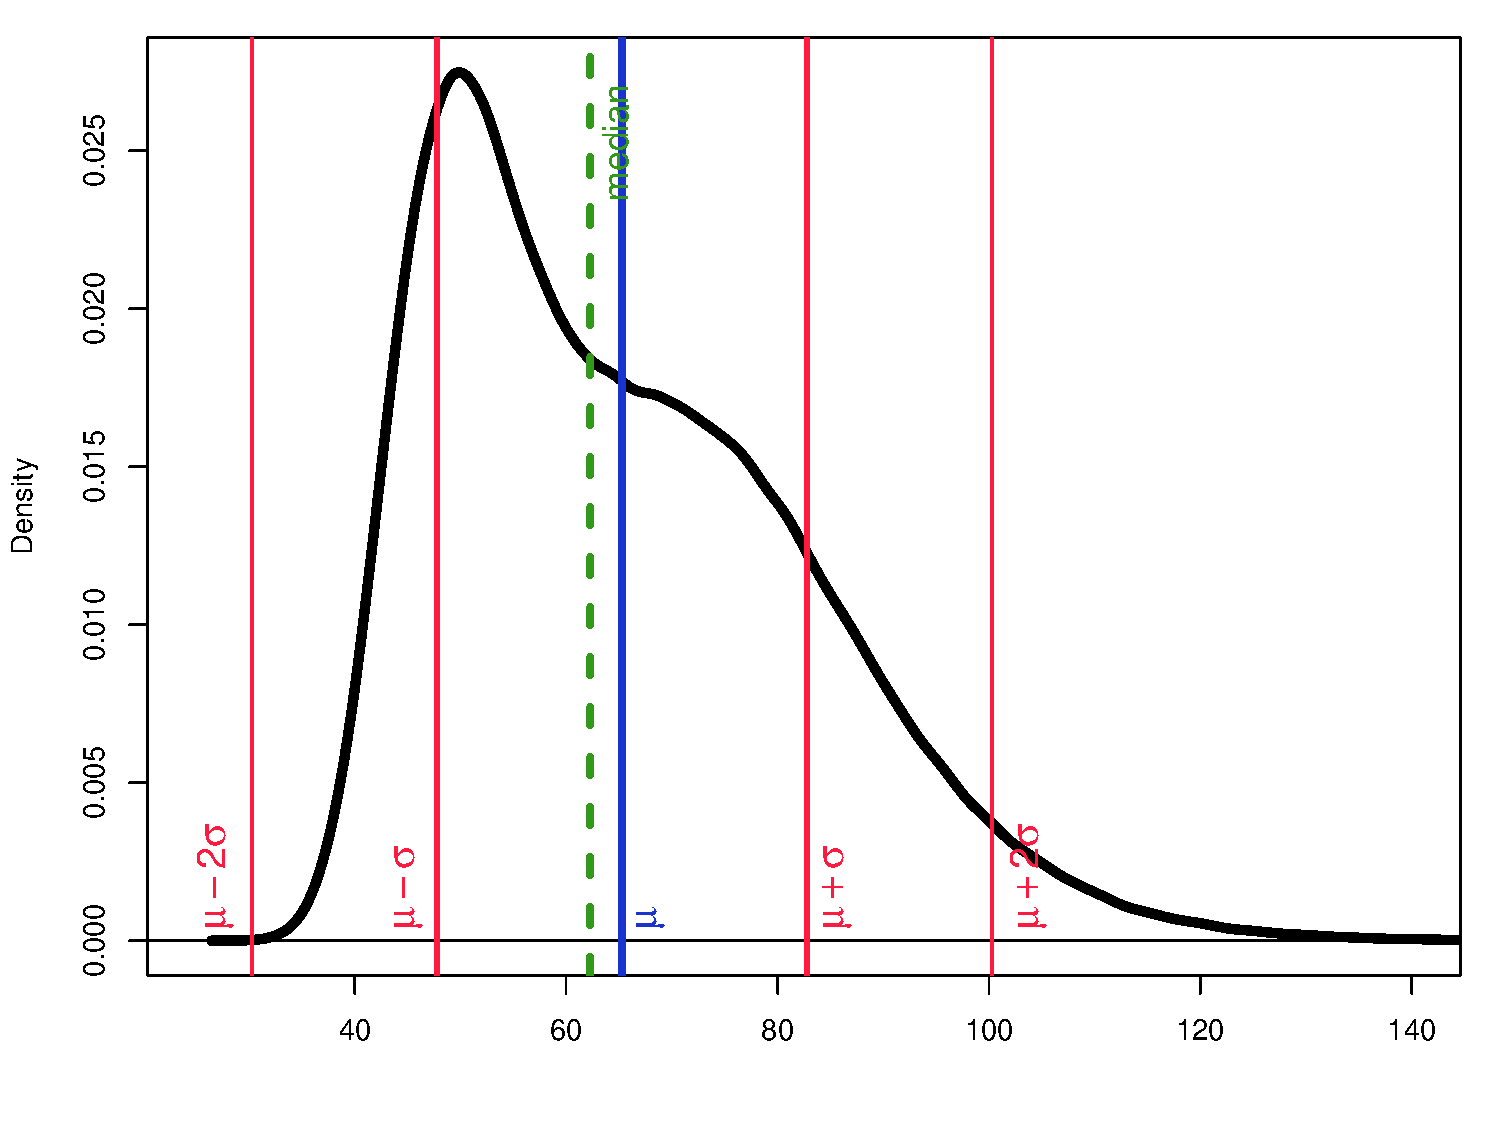
\includegraphics[width=9cm]{img/disttype_complicated}

    \ungap[1]
    \h{complicated \ldots}
  \end{center}
\end{frame}

\begin{frame}
  \frametitle{Different types of continuous distributions}
  
  \ungap[1]
  \begin{center}
    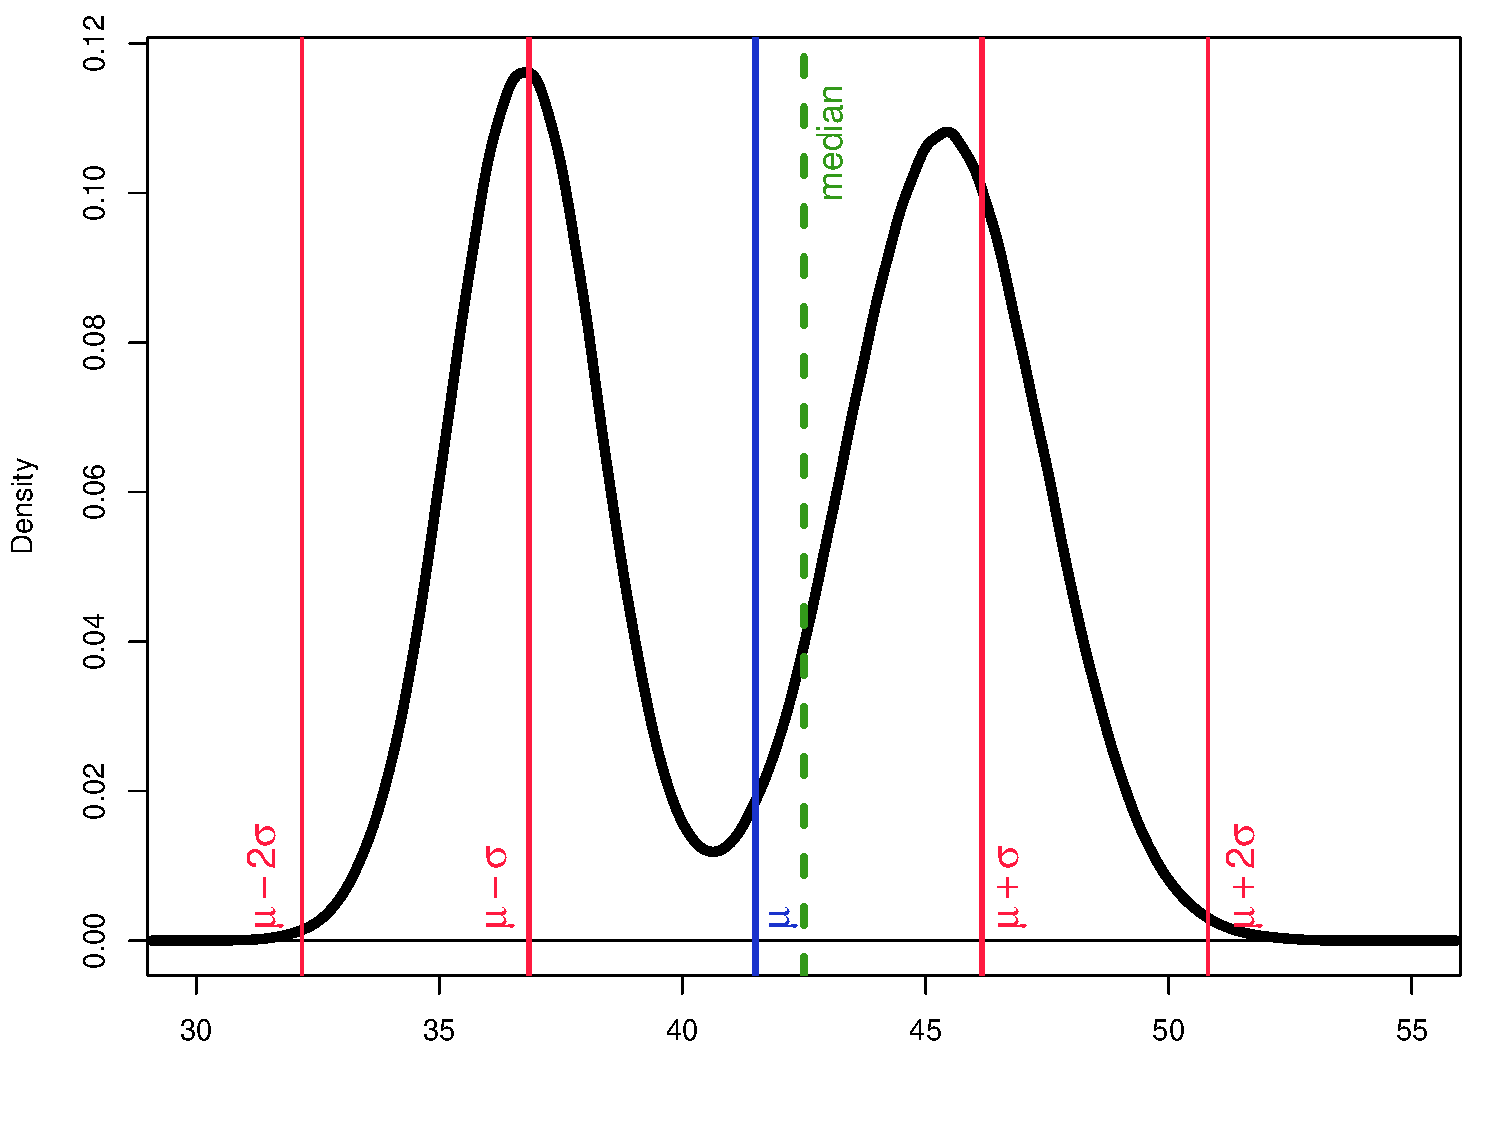
\includegraphics[width=9cm]{img/disttype_bimodal}

    \ungap[1]
    \h{bimodal} (mean \& median misleading)
  \end{center}
  \addnote{For each distribution type, ask participants how well the
    population is described by $\mu$ and $\sigma$.}%
  \addnote{Explain concepts of median and mode on these examples.}%
\end{frame}

%%%%%%%%%%%%%%%%%%%%%%%%%%%%%%%%%%%%%%%%%%
\subsection{The normal distribution (Gaussian)}

\begin{frame}
  \frametitle{The Gaussian distribution}
  % \framesubtitle{}

  \begin{itemize}
  \item In many real-life data sets, the distribution has a typical
    ``bell-shaped'' form known as a \h{Gaussian} (or \h{normal}) 
  \end{itemize}

  \pause
  \begin{center}
    \includegraphics[width=10cm]{img/gauss_10dm}
  \end{center}
\end{frame}

\begin{frame}
  \frametitle{}
  %% \framesubtitle{}

  \begin{itemize}
  \item Idealised density function is given by simple equation:
    \[
    g(t) = \frac{1}{\sigma \sqrt{2\pi}} e^{-(t-\mu)^2 / 2\sigma^2}
    \]
    with parameters $\mu\in\setR$ (location) and $\sigma > 0$ (width)
    \begin{center}
      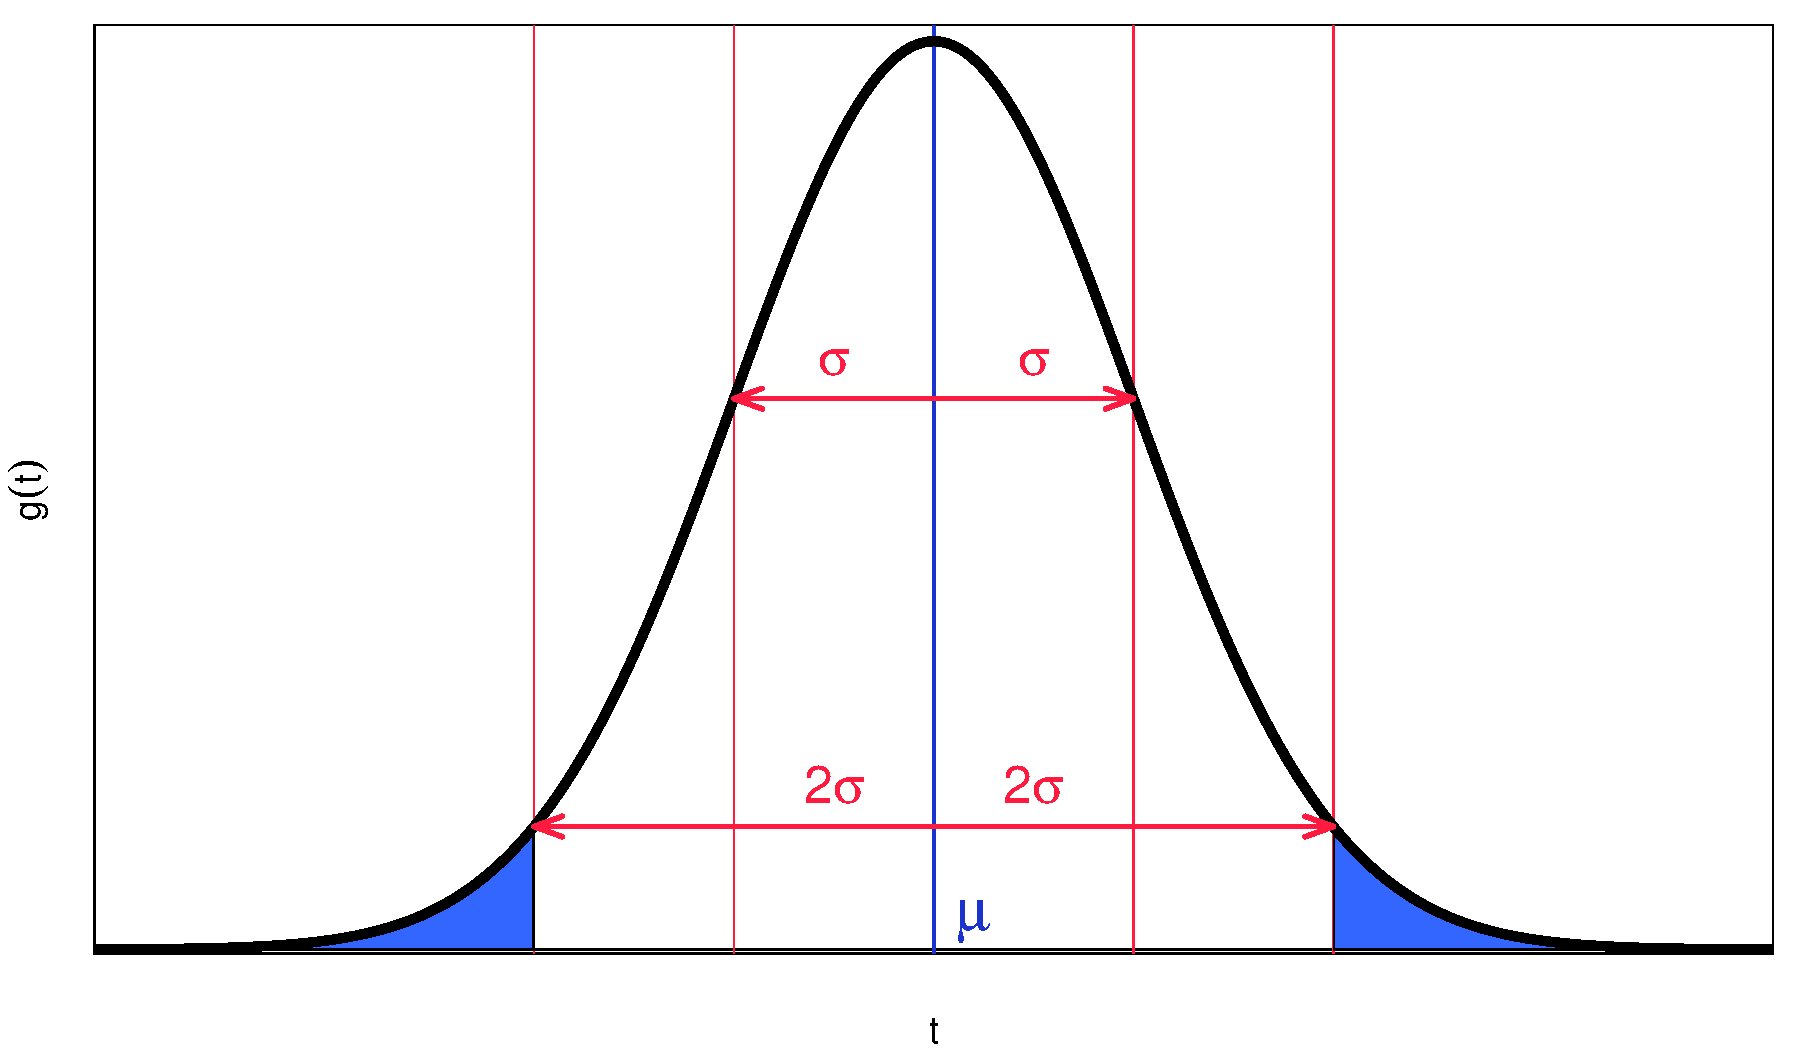
\includegraphics[width=8cm]{img/gaussian_parameters}
    \end{center}
  \item Notation: $X \sim N(\mu,\sigma^2)$ if r.v.\ has such a distribution
  \item No coincidence: $\Exp{X} = \mu$ and $\Var{X} = \sigma^2$ (\so homework ;-)
  \end{itemize}
\end{frame}

\begin{frame}
  \frametitle{Important properties of the Gaussian distribution}
  %% \framesubtitle{}

  \begin{itemize}
  \item<1-> Distribution is well-behaved: symmetric, and most values are
    relatively close to the mean $\mu$ (within 2 standard deviations)
    \begin{align*}
      \p{\mu-2\sigma\leq X\leq \mu+2\sigma} 
      &= \int_{\mu-2\sigma}^{\mu+2\sigma }
      \frac{1}{\sigma \sqrt{2\pi}} e^{-(t-\mu)^2 / 2\sigma^2} \dX{t}\\
      &\approx 95.5\%
    \end{align*}
    \ungap[1.5]
    \begin{itemize}
    \item 68.3\% are within range $\mu-\sigma\leq X\leq \mu+\sigma$
      (one s.d.)
    \item[]
    \end{itemize}
  \item<2-> The \h{central limit theorem} explains why this particular
    distribution is so widespread (sum of independent effects)
    \begin{itemize}
    \item[]
    \end{itemize}
  \item<3->[\hand] Mean and standard deviation are meaningful characteristics
    if distribution is Gaussian or near-Gaussian
    \begin{itemize}
    \item completely determined by these parameters
    \end{itemize}
  \end{itemize}
\end{frame}

\begin{frame}
  \frametitle{Assessing normality}
  
  \begin{itemize}
  \item Many hypothesis tests and other statistical techniques assume that
    random variables follow a Gaussian distribution 
    \begin{itemize}
    \item If this \h{normality assumption} is not justified, a significant
      test result may well be entirely spurious.
    \item[]
    \end{itemize}
  \item It is therefore important to verify that sample data come from such a
    Gaussian or near-Gaussian distribution
    \begin{itemize}
    \item[]
    \end{itemize}
    \pause
  \item Method 1: Comparison of histograms and density functions
    \begin{itemize}
    \item[]
    \end{itemize}
    \pause
  \item Method 2: Quantile-quantile plots
  \end{itemize}
\end{frame}

\begin{frame}<beamer:1-3| handout:1-2>
  \frametitle{Assessing normality: Histogram \& density function}
  
  \begin{columns}[c]
    \begin{column}{4cm}
      Plot histogram and estimated density:\\[0.5em]
      \begin{footnotesize}
        \secondary{\texttt{> hist(x,freq=FALSE)}}\\
        \secondary{\texttt{> lines(density(x))}}\\[1.5em]
      \end{footnotesize}
      \visible<2->{
        Compare best-matching Gaussian distribution:\\[0.5em]
        \begin{footnotesize}
          \secondary{\texttt{> xG <- seq(min(x),max(x),len=100)}}\\
          \secondary{\texttt{> yG <- dnorm(xG,mean(x),sd(x))}}\\
          \secondary{\texttt{> lines(xG,yG,col="red")}}\\[1.5em]
        \end{footnotesize}
      }
      \visible<beamer:3-| handout:2->{
        Substantial deviation \so\ not normal (problematic)
      }
   \end{column}
    \begin{column}{6cm}
      \only<beamer:1| handout:0>{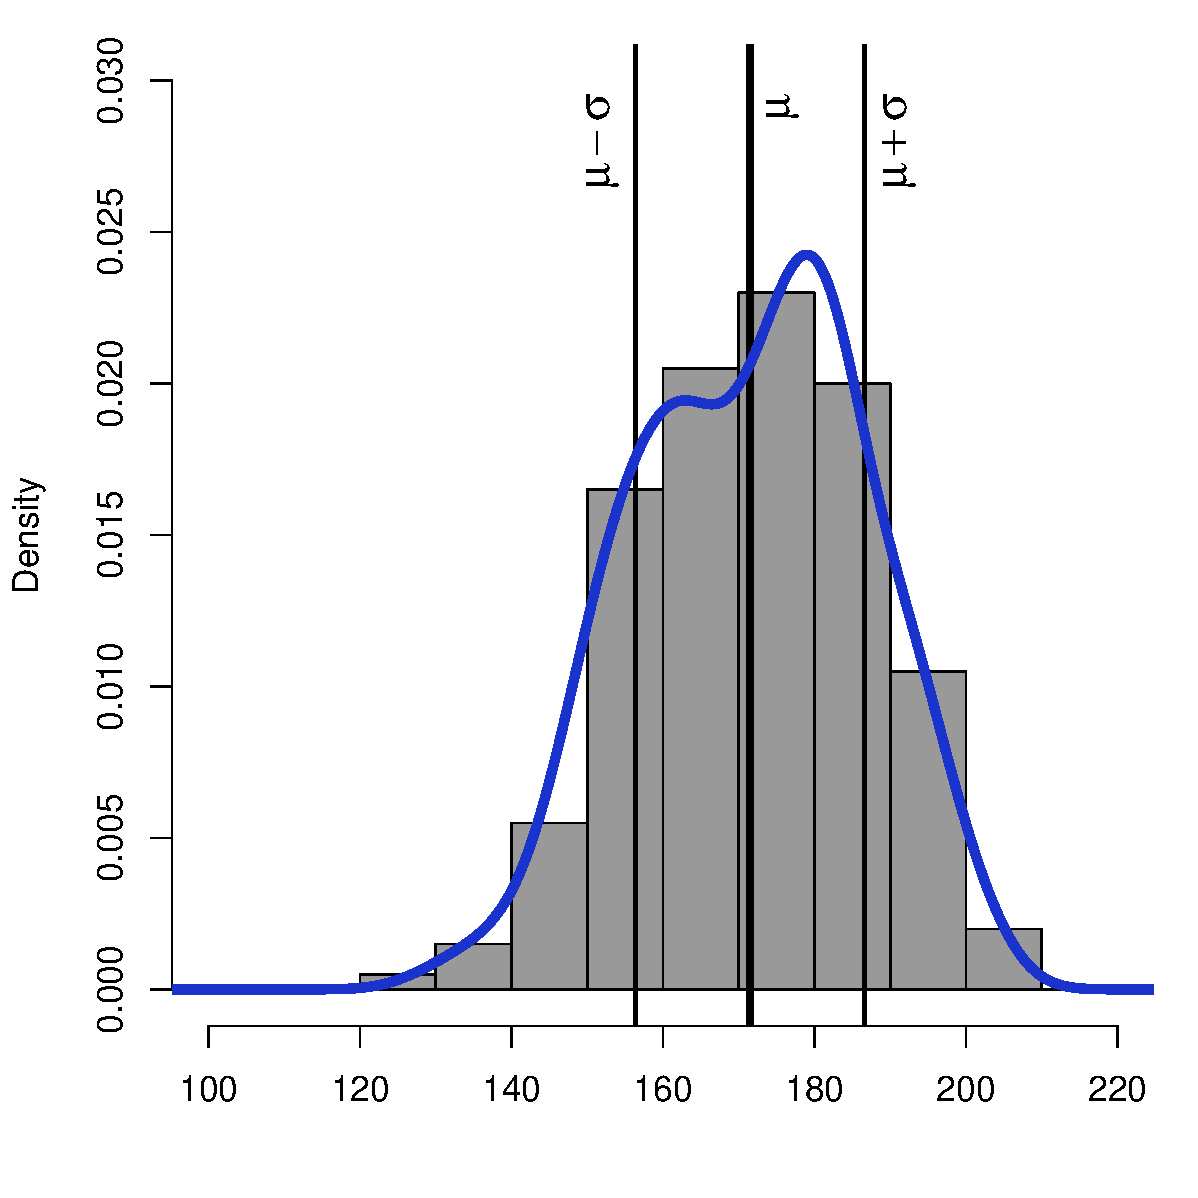
\includegraphics[width=6cm]{img/normality_bulgy_1}}%
      \only<beamer:2| handout:1>{\includegraphics[width=6cm]{img/normality_bulgy_2}}%
      \only<beamer:3| handout:2>{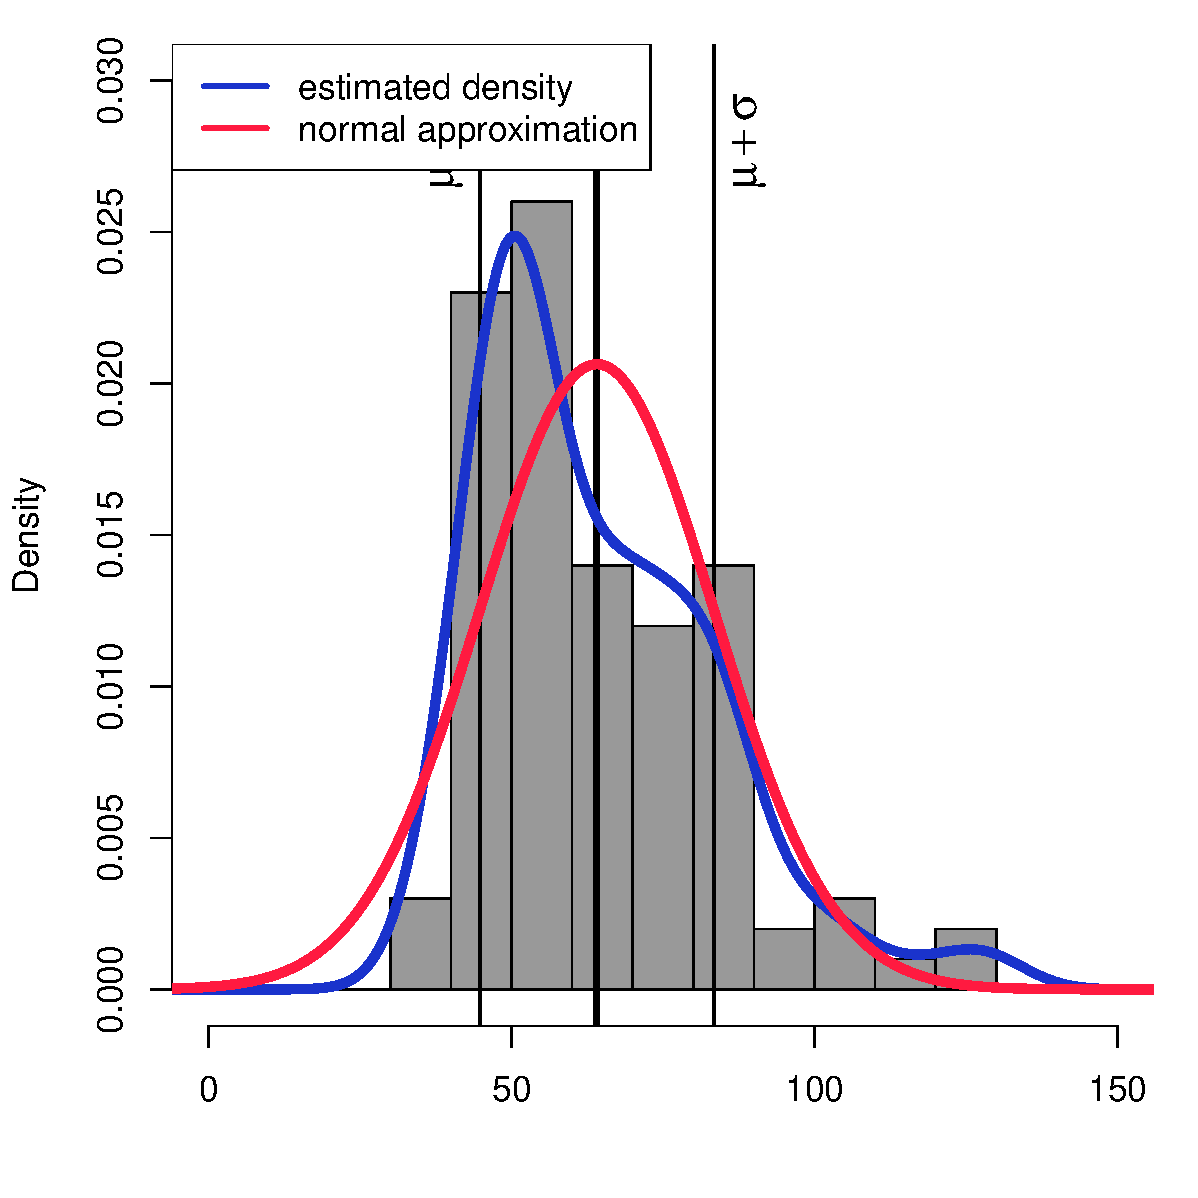
\includegraphics[width=6cm]{img/normality_complicated}}%
    \end{column}
  \end{columns}
\end{frame}

\begin{frame}<beamer:1-2| handout:1-2>
  \frametitle{Assessing normality: Quantile-quantile plots}
  
  \begin{columns}[c]
    \begin{column}{4cm}
      Quantile-quantile plots are better suited for small samples:\\[0.5em]
      \begin{small}
        \secondary{\texttt{> qqnorm(x)}}\\
        \secondary{\texttt{> qqline(x,col="red")}}\\[1.5em]
      \end{small}
      If distribution is near-Gaussian, points should follow red line.\\[1.5em]
      \visible<2->{
        One-sided deviation\\ \so\ skewed distribution
      }
   \end{column}
    \begin{column}{6cm}
      \only<beamer:1| handout:1>{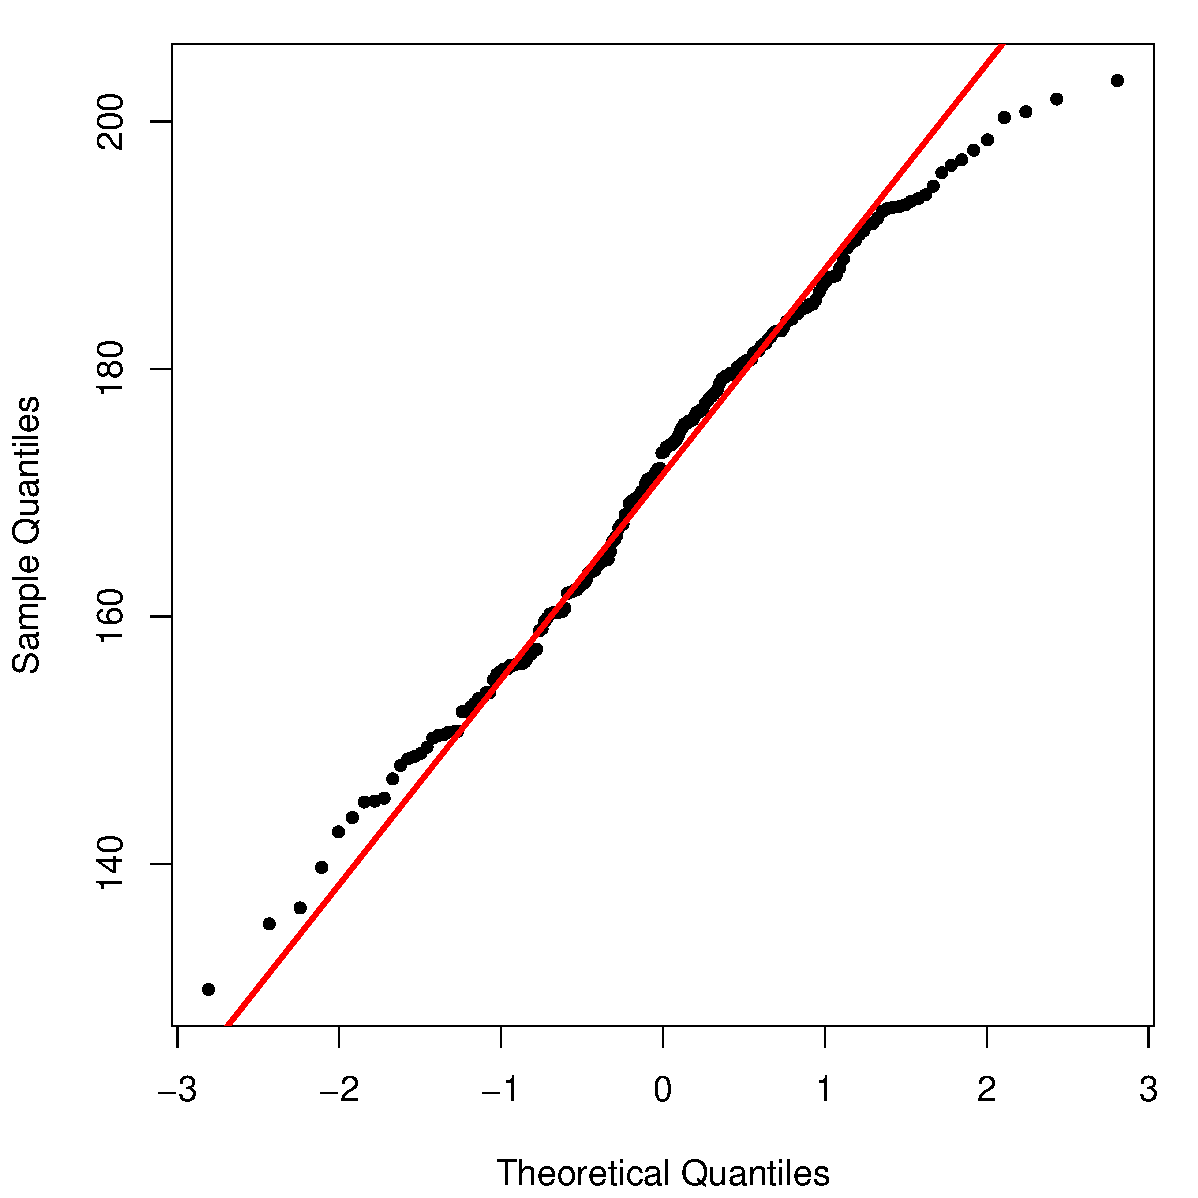
\includegraphics[width=6cm]{img/qqnorm_bulgy}}%
      \only<beamer:2| handout:2>{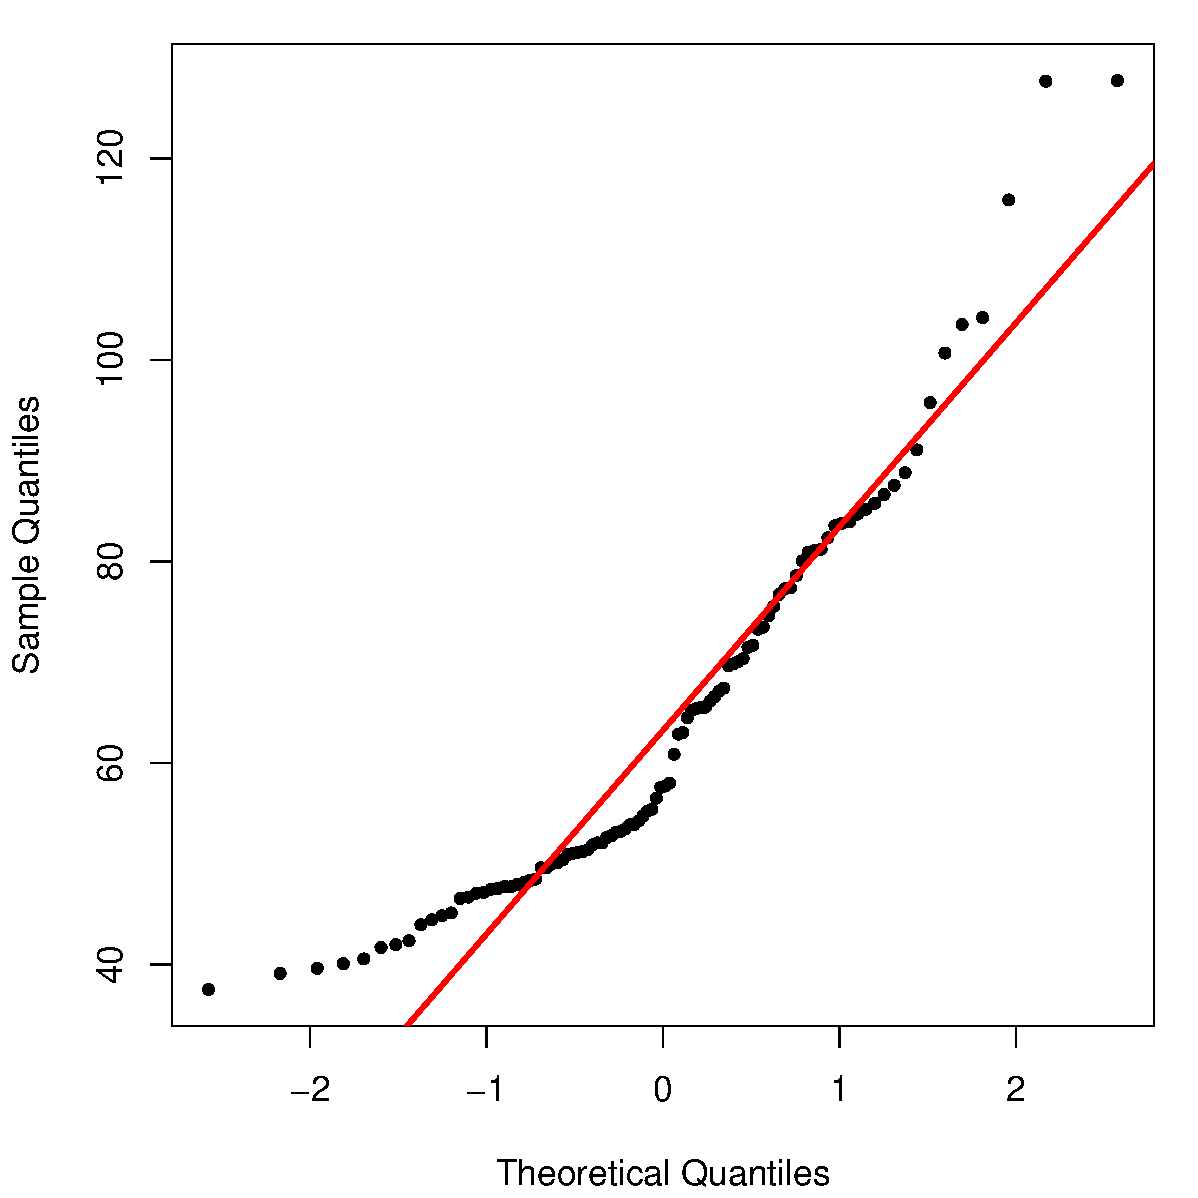
\includegraphics[width=6cm]{img/qqnorm_complicated}}%
    \end{column}
  \end{columns}
\end{frame}

\begin{frame}[fragile]
  \frametitle{Playtime!}
  \begin{itemize}
  \item Take random samples of $n$ items each from the census and wikipedia
    data sets (e.g.\ $n=100$)
    \begin{alltt}\color{secondary}
     library(corpora)
     Survey <- sample.df(FakeCensus, \emph{\primary{n}}, sort=TRUE)\end{alltt}
  \item Plot histograms and estimated density for all variables
  \item Assess normality of the underlying distributions
    \begin{itemize}
    \item by comparison with Gaussian density function
    \item by inspection of quantile-quantile plots
    \item[\hand] Can you make them look like the figures in the slides?
    \end{itemize}
  \item Plot histograms for all variables in the full data sets\\
    (and estimated density functions if you're patient enough)
    \begin{itemize}
    \item What kinds of distributions do you find?
    \item Which variables can meaningfully be described by\\
      mean $\mu$ and standard deviation $\sigma$?
    \end{itemize}
  \end{itemize}
\end{frame}

%%%%%%%%%%%%%%%%%%%%%%%%%%%%%%%%%%%%%%%%%%%%%%%%%%%%%%%%%%%%%%%%%%%%%%
%% References (if any)

%% \frame[allowframebreaks]{
%%   \frametitle{References}
%%   \bibliographystyle{natbib-stefan}
%%   \begin{scriptsize}
%%     \bibliography{sigil}
%%   \end{scriptsize}
%% }

\end{document}
